%%%%%%%%%%%%%%%%%%%%%%%%%%%%%%%%%%%%%%%%%%%%%%%%%%%%%%%%%%%%%%%%%%%%%%%%%%%%%%%%
% 05_scales_and_smearings.tex: Derivation of the scales and smearings
%%%%%%%%%%%%%%%%%%%%%%%%%%%%%%%%%%%%%%%%%%%%%%%%%%%%%%%%%%%%%%%%%%%%%%%%%%%%%%%%
\chapter{Measurement of the energy scale and resolution of the CMS ECAL}
\label{chap:scales}
%%%%%%%%%%%%%%%%%%%%%%%%%%%%%%%%%%%%%%%%%%%%%%%%%%%%%%%%%%%%%%%%%%%%%%%%%%%%%%%%

%%%%%%%%%%%%%%%%%%%%%%%%%%%%%%%%%%%%%%%%%%%%%%%%%%%%%%%%%%%%%%%%%%%%%%%%%%%%%%%%

\section{Introduction}

The precise calibration of the CMS ECAL is essential in making a precision mass of the Higgs boson measurement in the diphoton channel. This chapter focuses on the calibration of the ECAL, with detailed descriptions of the setting of the energy scale and the procedure for matching the resolution in simulation with the observed resolution in the data. 

First, the need for residual energy scales and additional Gaussian smearings is motivated by discussing various detector features that affect the energy scale and resolution. Then, these detector properties are summarized by measurements of Z$\rightarrow ee$ events. A method of correcting the residual differences in energy scale and resolution between data and simulation was developed in 2012 and is described in Ref~\cite{Nourbakhsh:1969408}. From this method, a modern technique to correct these residual differences was developed that relies on the increased data in Run 2. Residual energy scale corrections and additional smearings from this new technique are incorporated in the H$\rightarrow\gamma\gamma$ analysis. Finally, the results of the method are demonstrated through the agreement of the dielectron invariant mass distribution in data and simulation.

\section{The energy resolution of the CMS ECAL}

The intrinsic energy resolution of the CMS ECAL, as measured in a test beam, takes the form:

\begin{equation}
    \frac{\sigma(E)}{E} = \frac{2.8\%}{\sqrt{E}} \oplus \frac{12\%}{E} \oplus 0.3\%
\end{equation}

\noindent where $E$ is the energy of an interacting particle in GeV, and $\sigma$ is the energy resolution. The three components represent, in order, the stochastic term due to fluctuations in the electromagnetic shower development, the noise term due to electronic noise, and the constant term due to a lack of full containment of the shower. These terms form the basis of the energy resolution of the CMS ECAL. However, additional factors affect the energy scale and resolution of the CMS ECAL, including the stability of the time response corrections, the precision of the inter-calibration corrections, and interactions with upstream material.

\subsection{Stability of the time response corrections}

The scintillation response of an ECAL crystal is related to its laser response via:
\begin{equation}
    \frac{S(t)}{S_0} = \left( \frac{R(t)}{R_0}\right)^{\alpha}
\end{equation}

\noindent where $S(t)$ is the scintillation response of the crystal at time $t$, $S_0$ is the initial scintillation response of the crystal, $R(t)$ is the laser response of the crystal at time $t$, $R_0$ is the initial laser response of the crystal, and $\alpha$ is a material dependent quantity. The value of $\alpha$ encodes both properties of the crystals themselves, such as roughness, transition, and manufacturing quality, as well as properties of the photodetectors used to read the scintillation light from the crystals, such as dark currents in the APDs, and the response loss of the VPTs due to irradiation. The value of $\alpha$ is fixed in the EB based on average values measured by monitoring the drift of the observed mass of the $\pi^0$. In the EE, $\alpha$ is derived as a function of location in the detector to account for the effect of increased crystal irradiation at high values of $|\eta|$ by monitoring the time stability of the mass of the Z boson. These corrections work well enough to ensure the relative energy resolution on the mass of the Z boson is around 0.1\% in the EB and between 0.1\% and 0.3\% in the EE. Since they are time-dependent, these corrections are applied only to data. Simulation does not account for any effects due to the irradiation of ECAL crystals. Therefore, the relative energy response in simulation is smaller than in data.

\subsection{Inter-calibration precision}

Due to natural variations in the manufacturing process, each crystal's response in the ECAL is slightly different. These variations in the response are corrected using a set of corrections known as inter-calibrations. 

To derive these inter-calibrations constraints from $\pi^0/\eta \rightarrow \gamma\gamma$ events, momentum constraints from Z and W decays, and the Z mass constraint in $Z\rightarrow ee$ decays are used to align the response and resolution of each crystal in the ECAL. The precision of the inter-calibrations for the Run 2 datasets is less than $\sim$0.5\% in the EB and less than 1\% in the EE. Variation with $\eta$ for the different years of data taking is shown in Figure~\ref{fig:ic_precision}. The inter-calibration precision contributes to the constant term of the energy resolution and is included in the simulation as a Gaussian mis-calibration to the crystal response.

\begin{figure}[h]
    \centering
    \includegraphics[width=\textwidth]{05-figures/final_Precision_RunII.png}
    \caption[Inter-calibration precision]{Precision of the inter-calibration procedure for the Run 2 datasets.}
    \label{fig:ic_precision}
\end{figure}

\subsection{Interaction with the upstream material}

It is essential to understand the amount of material between the ECAL and the interaction point for precise energy and resolution calibration. Electromagnetic objects may interact with this upstream material, beginning their shower development before reaching the ECAL. The amount of material between the ECAL and the interaction point, as implemented in the simulation of the CMS detector, is shown in Figure~\ref{fig:upstream_material}. In the case of an upstream interaction, some energy will inevitably be lost before the ECAL. The shower shape variable $R_9$ is the ratio of energy deposited in the core of an electromagnetic shower to the total energy measured from the shower. It reflects how strongly an electron or photon has interacted upstream of the ECAL and, thus, how much energy it has lost in transit. A threshold at $R_9 = 0.96$ is set to divide low-bremsstrahlung objects from high-bremsstrahlung objects, or those without significant upstream interactions and those with substantial upstream interactions. Though good, the simulation of the ECAL is not perfect, and differences in the model of the upstream material and the ECAL itself contribute to residual differences in the energy resolution of data and simulation. 

\begin{figure}[h]
    \centering
    \includegraphics[width=0.5\textwidth]{05-figures/Tracker_SubDetectors_x_vs_eta.png}
    \caption[Material budget]{The amount of material between the ECAL and the interaction point measured in radiation lengths $\chi_0$ as a function of pseudorapidity.}
    \label{fig:upstream_material}
\end{figure}

\section{The energy scale and resolution of electrons in the CMS ECAL}

The energy scale and resolution of objects in the CMS ECAL have been described now as a function of time, position in the detector of the reconstructed object, and the shower shape variable R$_9$ associated with the object. These effects are monitored closely, and the stability of the scale of reconstructed Z bosons and the stability of the R$_9$ of the leading electron in Z$\rightarrow ee$ events are shown in Figures~\ref{fig:z_mass_stability} and ~\ref{fig:r9_stability} for events across all of Run 2.

\begin{figure}[h]
    \centering
    \includegraphics[width=\textwidth]{05-figures/final_medianmeevstimeinEB_rotate.png}
    \caption[Dielectron invariant mass stability]{The time stability of the median dielectron invariant mass for the full Run 2 dataset. Both electrons are required to be in the ECAL barrel. Each time bin has around 10,000 events. The error bar on the points denotes the statistical uncertainty on the median, which is evaluated as the central 95\% interval of medians obtained from 200 ``bootstrap" re-samplings. The right panel shows the distribution of the medians.}
    \label{fig:z_mass_stability}
\end{figure}

\begin{figure}[h]
\subfloat{%
    \begin{minipage}[t]{0.49\textwidth}%
        \centering
        \includegraphics[width=\textwidth]{05-figures/final_medianR9eLvstimeinEB_rotate.png}
    \end{minipage}
    }~\subfloat{%
    \begin{minipage}[t]{0.49\textwidth}%
        \centering
        \includegraphics[width=\textwidth]{05-figures/final_medianR9eLvstimeinEE_rotate.png}
    \end{minipage}
    }
    \centering
    \caption[R$_9$ stability in Run 2]{The time stability of the shower shape of the leading electron in Z decays for the full Run2 dataset. The event selection requires two electrons in the ECAL Barrel and two in the ECAL Endcaps on the left and right, respectively. Each time bin has around 10,000 events. The error bar on the points denotes the statistical uncertainty on the median, which is evaluated as the central 95\% interval of medians obtained from 200 ``bootstrap" re-samplings. The right panel shows the distribution of the medians. The shower shape is measured by the variable R$_9$.}
    \label{fig:r9_stability}
\end{figure}

The relative energy resolution of the CMS ECAL in Run 2 measured through Z$\rightarrow ee$ decays is shown in Figure~\ref{fig:run2_resolution} for the case low bremsstrahlung electrons and the inclusive case.

\begin{figure}[h]
    \subfloat{%
    \begin{minipage}[t]{0.49\textwidth}%
        \centering
        \includegraphics[width=\textwidth]{05-figures/final_Resolution_RunII_Inclusive.png}
    \end{minipage}
    }~\subfloat{%
    \begin{minipage}[t]{0.49\textwidth}%
        \centering
        \includegraphics[width=\textwidth]{05-figures/final_Resolution_RunII_LowBremsstrahlung.png}
    \end{minipage}
    }
    \centering
     \caption[Relative resolution of electrons in Run 2]{Relative electron energy resolution in bins of pseudorapidity $\eta$ for the ECAL Barrel and Endcap measured using Z$\rightarrow ee$. The resolution is shown separately for low bremsstrahlung electrons (right) and all electrons (left). The plot compares the resolution achieved after a refined calibration of the data collected at 13 TeV during Run 2 in 2016, 2017, and 2018.}
    \label{fig:run2_resolution}
\end{figure}

There are residual differences between data and simulation in both the scale and the width of the dielectron invariant mass distributions, even after reconstruction and initial corrections. Examples of the agreement after reconstruction are shown in Figure~\ref{fig:ul17_raw}. 

\begin{figure}[h]
    \subfloat{%
    \begin{minipage}[t]{0.49\textwidth}%
        \centering
        \includegraphics[width=\textwidth]{05-figures/money_2017_ul_Raw_EbEb_inclusive_wRatioPad.png}
    \end{minipage}
    }~\subfloat{%
    \begin{minipage}[t]{0.49\textwidth}%
        \centering
        \includegraphics[width=\textwidth]{05-figures/money_2017_ul_Raw_EeEe_inclusive_wRatioPad.png}
    \end{minipage}
    }
    \centering
     \caption[Dielectron invariant mass distributions after reconstruction and electron energy regression]{Dielectron invariant mass distributions in 2017 data and simulation requiring two electrons in the ECAL barrel (left) and two electrons in the endcap (right). These plots show the residual differences in the energy scale and resolution of the distributions after reconstruction and application of the electron energy regression.}
    \label{fig:ul17_raw}
\end{figure}

\subsection{Z$\rightarrow e^+e^-$ event selection}

\subsubsection{Trigger}

The trigger menu cuts are described in Table~\ref{tab:double_eg_trigger} and are identical to the diphoton events cuts.

\subsubsection{Offline selection}

Events used in this analysis are required to have passed the selected trigger, and dielectron events must fulfill the following additional requirements:

\begin{itemize}
    \item Leading and subleading electrons must have an $E_T > 32$ and $E_T > 20$ respectively
    \item Both electrons must pass the loose electron identification and isolation criteria
    \item Both electrons must be in the ECAL fiducial region, with both electrons in the tracker acceptance ($|\eta| < 2.5$), with a veto applied to electrons near the barrel transition region, meaning $1.4442 < |\eta| < 1.566$. 
\end{itemize}

Events must also satisfy cuts on kinematic variables in the CMS standard electron identification criteria:

\begin{itemize}
    \item $\Delta\eta$: The difference in pseudorapidity between the measured track associated with the electron and the vertex and the center of the ECAL cluster extrapolated to the vertex.
    \item $\Delta\phi$: The difference in the angle in transverse with respect to the beam axis between the measured track of an electron at the vertex and the center of the ECAL cluster extrapolated to the vertex.
    \item $\sigma_{i\eta i\eta}$: A shower shape variable defined as \begin{equation*} \sigma_{i\eta i\eta} = \sqrt{\frac{\sum (\eta_i - \overline{\eta})^2 w_i}{\sum w_i}}\mathrm{, where \ } \overline{\eta} = \frac{\sum w_i \eta_i}{\sum w_i} \mathrm{\ and \ } w_i = \max\left( 0, 4.7 + \log\left(\frac{E_i}{E_{5\times 5}}\right) \right) \end{equation*} where the sum runs over the $5\times 5$ crystal matrix around the crystal in the cluster containing the largest deposited energy, and the $\eta$ distances are measured in units of the size of the crystals in the $\eta$ direction.
    \item $H/E$: The ratio of the energy deposited in the HCAL in a cone of $\Delta R = 0.15$ centered around the seed of the ECAL cluster to the energy deposited in the ECAL.
    \item Impact Parameters: The dielectron vertex position is compared with the closer primary vertex in the transverse plan with respect to the beam axis ($d0(vtx)$) and in the beam axis direction ($dz(vtx)$).
    \item $|1/E - 1/p_{in}|$: The absolute difference between the inverse of the supercluster energy and the inverse of the track momentum at the vertex.
    \item PFiso: Based on the particle flow algorithm, the isolation variable is defined as a combination of the activity of charged and neutral particles around the considered electron after removing the electron deposit.
    \item Conversion rejections: Two cuts are used to reject converted photons: the vertex fit probability must be below 1e$-6$, and the number of missing points in a reconstructed track is constrained to be one or fewer.
\end{itemize}

The criteria for each of these variables are defined for different efficiencies and purities and are summarized in Table~\ref{tab:electron_event_selection_cuts}.

\begin{table}[h]
    \centering
    \begin{tabular}{|c||c|c|c||c|c|c|}
         \hline
         Variable & \multicolumn{6}{c|}{Cut Thresholds} \\
         & \multicolumn{3}{c||}{EB} & \multicolumn{3}{c|}{EE} \\ \hline
         & loose & medium & tight & loose & medium & tight \\ \hline \hline
         & \multicolumn{6}{c|}{Electron Identification Variables} \\ \hline
         $|\Delta\eta| <$ & 0.007 & 0.004 & 0.004 & 0.009 & 0.007 & 0.005 \\ \hline
         $|\Delta\phi| <$ & 0.15 & 0.06 & 0.03 & 0.10 & 0.03 & 0.02 \\ \hline
         $\sigma_{i\eta i\eta} <$ & \multicolumn{3}{c||}{0.01} & \multicolumn{3}{c|}{0.03} \\ \hline
         $H/E <$ & \multicolumn{3}{c||}{0.12} & \multicolumn{3}{c|}{0.10} \\ \hline
         $|1/E - 1/p_{in}| <$ & \multicolumn{3}{c||}{0.05} & \multicolumn{3}{c|}{0.05} \\ \hline
         & \multicolumn{6}{c|}{Impact Parameters} \\ \hline
         $|d0(vtx)| < $ & \multicolumn{3}{c||}{0.02} & \multicolumn{3}{c|}{0.02} \\ \hline
         $|dZ(vtx)| < $ & 0.2 & \multicolumn{2}{c||}{0.01} & 0.2 & \multicolumn{2}{c|}{0.01} \\ \hline
         & \multicolumn{6}{c|}{Electron Isolation Variable} \\ \hline
         PFIso / $p_T$ ($\Delta R = 0.3$) $<$ & \multicolumn{2}{c|}{0.15} & 0.10 & \multicolumn{2}{c|}{0.15} & 0.10 \\ \hline
         & \multicolumn{6}{c|}{Conversion Rejection Variables} \\ \hline
         Vtx. Fit Prob. & \multicolumn{3}{c||}{1e-6} & \multicolumn{3}{c|}{1e-6} \\ \hline
         Missing Hits $\leq$ & \multicolumn{2}{c|}{1} & 0 & \multicolumn{2}{c|}{1} & 0 \\ \hline 
    \end{tabular}
    \caption[Electron selection criteria and cut thresholds]{Electron selection criteria and cut thresholds for the EB and EE are shown for three working points (loose, medium, and tight) corresponding to 90\%, 80\%, and 70\% selection efficiency, respectively. The purity of the electron sample will increase as the selection efficiency decreases.}
    \label{tab:electron_event_selection_cuts}
\end{table}

The primary sources of background found in these events come from electroweak processes like $W\rightarrow\ell\nu$, and $Z\rightarrow\tau\tau$, and QCD events, including $t\overline{t}$ events. The loose working point has an efficiency of around 90\% and contains negligible background.

\subsection{Simulation}

Two large simulated MC samples are used for the $Z\rightarrow ee$ signal. These are summarized in Table~\ref{tab:drell-yan_simulation}.

\begin{table}[h]
    \centering
    \begin{tabular}{|c|c|c|c|}
        \hline
        Year & Process & Generator & $\sqrt{s}$ \\ \hline \hline
        2016 & Drell-Yan to leptons & AMC@NLO & 13 TeV \\ \hline
        2017 & Drell-Yan to leptons & MadGraph + AMC@NLO & 13 TeV \\ \hline
        2018 & Drell-Yan to leptons & MadGraph + AMC@NLO & 13 TeV \\ \hline
    \end{tabular}
    \caption[Simulation samples for Run 2]{Simulation samples used as signal in 2016, 2017, and 2018 for $Z\rightarrow ee$ events.}
    \label{tab:drell-yan_simulation}
\end{table}


\subsection{Comparison of data and MC samples}

Previous studies have shown differences in the shapes of the $p_T(Z)$ and rapidity ($y(Z)$) distributions in data and the above simulation. These differences are corrected using weight factors derived in bins of $p_T(Z)$ and $y(Z)$. The weights ensure that the shapes of these distributions match. First, a 2D histogram of event counts is created in the $p_T(Z)$ and $y(Z)$ space in both simulation and data. The histograms are normalized to preserve the total event count after reweighting. The weights are calculated by dividing the normalized number of events in the data by the normalized number of events in the simulation. Then, by applying these weights to the simulation, the shape of $p_T(Z)$ and $y(Z)$ will match that in the data. The bins in which the scale factors were derived are:

\begin{itemize}
    \item If $p_T(Z) < 40$ GeV then the bin sizes are 1 GeV, otherwise $[40, 45, 50, 55, 60, 80, 100, > 100]$
    \item $y(Z)$: $[0, 0.3, 0.6, 0.9, 1.2, 1.5, 1.7, 1.8, 2.1, 2.3, 2.5]$, and similarly for negative $y(Z)$.
\end{itemize}

\section{The global smearing method}
\label{sec:gsm}

The global smearing method (GSM) aligns the scale of the dielectron invariant mass peak in data with the scale of the dielectron invariant mass peak in simulation and applies additional Gaussian smearing to the dielectron invariant mass distribution in simulation to match the resolution of the same distribution in data. This method is described in detail in this section. 

\subsection{Framework outline}

The GSM framework is a suite of tools built in Python whose primary purpose is to improve the agreement in data and simulation by minimizing a loss function built around the negative log-likelihood, and reducing the difference between data and simulation in categories defined in terms of single electron properties. SciPy's Optimize package handles the minimization and implements the L-BFGS-B method: a limited memory, bounded, hill climbing algorithm that is robust and fast for large phase spaces \cite{byrd_lu_nocedal_zhu_1995,zhu_byrd_lu_nocedal_1997,morales_nocedal_2011}. The general outline of the framework, with more details on each step provided in subsequent sections below, is as follows:

\begin{itemize}
    \item define $n$ scale categories and $k$ smearing categories based on single electron properties such as location in the detector ($|\eta|$), the probability of having had an upstream interaction ($R_9$), and transverse energy ($E_T$).
    \item Associate a scale with each scale category $n$, and a Gaussian width with each smearing category $k$.
    \item Construct $n(n+1)/2$ dielectron invariant mass distributions in both data and simulation where each distribution contains events with electrons from two, and only two, single electron scale categories $n$ and $m$, and two smearing categories $k$ and $l$.
    \item Evaluate a loss function across all dielectron invariant mass categories (($n$,$j$),($k$,$l$)) 
    \item Provide the loss function to SciPy's minimize tool in the Optimize sub-library and allow the minimizer to find values of all $n$ scales and all $k$ Gaussian widths for the smearing categories.
\end{itemize}

The framework improves the agreement between data and simulation in a series of compounded steps, with the binning becoming progressively finer. The different steps are as follows:

\begin{itemize}
    \item Run number $\times$ $|\eta|$: The first step uses the ``median method" (described in detail below) to correct the median invariant mass to that in simulation in bins of run number, and $|\eta|$ which stabilizes the dielectron invariant mass distribution in time and location in the detector.
    \item $|\eta| \times R_9$: The next step uses the GSM's minimization procedure to derive both the residual scales and additional smearings simultaneously in bins of $|\eta|$ and $R_9$ using electrons that have already been corrected using the scales derived in the previous step. This compounding effect further improves the agreement between data and simulation. From now on, this compounded process will be referred to as ``on top of", i.e., a new set of scales is derived \textit{on top of} a previous set of scales. The bins are coarse, with four bins in $|\eta|$, as in the last step, and two bins in $R_9$, where the divide between bins separates low-bremsstrahlung and high-bremsstrahlung electrons.  
    \item Granular $|\eta| \times R_9$: The minimization procedure is used to derive the residual scales and additional smearings simultaneously in bins of $|\eta|$ and $R_9$. In this step, the smearings are rederived as the bins remain coarse with four bins in $|\eta|$ and two bins in $R_9$. The granular $|\eta| \times R_9$ scales are derived on top of the $|\eta| \times R_9$. The bins sizes are much more granular than in the previous step, with five bins in $|\eta|$ and between 8 and 16 bins in $R_9$.
    \item $|\eta| \times E_T$: In this step, a set of residual scales are derived on top of the results from the previous step in 5 bins of $|\eta|$ and between 4 and 10 bins in electron $E_T$. 
    \item $|\eta| \times E_T$: This step derives a set of residual scales \textit{and} additional smearings in 4 bins of $|\eta|$, two bins of $R_9$, and four bins of electron $E_T$. The scales are derived on top of the previous results.
    
\end{itemize}

\subsection{The ``median method"}

The ``median method" is used to derive the first set of corrections, which stabilize the dielectron invariant mass distribution in time and location in the detector. Dielectron invariant mass distributions are built for each run bin, defined as a group of runs with a minimum of 10,000 dielectron events, and are divided into four bins in $|\eta|$. The scale for each category is the factor that corrects the median of the dielectron invariant mass distributions to the PDG value of the mass of the Z boson:

\begin{equation}
    \mathrm{scale}^{\mathrm{run\ bin}} = 91.188 \mathrm{\ GeV} / \text{median}(M_{ee}^{\mathrm{run\ bin}}).
\end{equation}

\subsection{Dielectron event categorization}

The GSM is used to derive corrections to single electron energies by scaling the energy of electrons in data to match the known value of the Z mass of 91.188 GeV \cite{pdg} in simulation, and to derive an additional Gaussian smearing to be applied to electrons in simulation to match the resolution in data. The GSM uses simulated Z boson decays as a template PDF for the data. This template approach accounts for known detector effects, reconstruction inefficiencies, and the kinematic behavior of the Z boson.

The categorization of the dielectron invariant mass is defined by $n$ categories based on single electron properties. This categorization approach produces $n(n+1)/2$ dielectron invariant mass categories ($D$ for data categories and $S$ for simulation categories). Each category is associated with two electron energy scales ($\Delta P_n$, $\Delta P_m$) applied to the energy of electrons in data and two electron energy smearings ($\Delta \sigma_k$, $\Delta \sigma_l$) applied to the energy of electrons in simulation ($D_{n,m}$ and $S^{k,l}_{n,m}$).\footnotemark\footnotetext{It is essential to note that all scale categories ($n,m$) are contained in the broader smearings categories ($k,l$) and that both data and simulation are categorized by ($n,m$)} The smearings are a multiplicative factor obtained from a random sampling of a Gaussian distribution of width $\Delta \sigma$ centered around 1, and cause the width of the dielectron invariant mass distribution in simulation to increase, since the width of the dielectron invariant mass distribution in simulation is always less than the width of that in data, by construction. The invariant mass distributions in the simulation are over-sampled to smooth the distributions after applying the additional Gaussian smearings and to increase the sensitivity of the additional smearings impact on the loss function. Over-sampling is implemented by doubling the number of events in simulation in a given category until the number of events exceeds 50 times the number of events in data or 50,000 events, whichever is larger. If there is a very high statistics category in data, an upper limit on the over-sampling of simulation is set at $10^6$ events to reduce the computational time of the method.

Once all categories are constructed, low statistics categories are deactivated. In data, active dielectron categories must have more than ten events. In simulation, active diagonal ($n = m$) dielectron categories must contain at least 1000 events, and all active off-diagonal ($n \neq m$) dielectron categories must contain at least 2000 events.

\subsection{Dielectron invariant mass binning}
    
The loss function used to evaluate the agreement between data and simulation is an event-weighted, binned, negative log likelihood that is combined with the chi-squared test. The dielectron invariant mass histograms are built for data and simulation in each dielectron category constructed from single electron categories $n$ and $m$. The number of bins in each dielectron category is determined using the Freedman-Diaconis rule, which is defined as:
 
\begin{equation}
    N_{n,m} = min( \left \lfloor{ \frac{D_{n,m}^{1/3}}{2*IQR(M_{ee}^{data,n,m})}} \right \rfloor, \left \lfloor{ \frac{S_{n,m}^{1/3}}{2*IQR(M_{ee}^{sim,n,m})}} \right \rfloor )
\end{equation}

\noindent where $D_{n,m}$ is the number of events in the data dielectron invariant mass histogram, IQR is the inter-quartile range, $M_{ee}^{data,n,m}$ is the distribution of dielectron invariant mass events in category $(n,m)$ in data, $S_{n,m}$ is the number of events from the dielectron invariant mass histogram in simulation, and $M_{ee}^{sim,n,m}$ is the distribution of dielectron invariant mass events in category $(n,m)$ in simulation.
By default, each histogram is truncated, with a lower bound at 80 GeV and an upper bound at 100 GeV. If the tails of the dielectron invariant mass histograms in data and simulation show a large disagreement that skews the results, the bounds on the histograms are made tighter to allow the fit to focus on improving the agreement between data and simulation in the core of the dielectron invariant mass distribution. 

\subsection{Loss function}

The binned negative log-likelihood between data and simulation is defined as follows:
\begin{equation}
    NLL_{n,m} = -2 * \sum_{i = 1}^{N_{n,m}} d_{i} p_{n,m} log(m_{i} \sigma_{n,m}) + (D_{n,m} - d_{i} p_{n,m})  log(1 - m_{i} \sigma_{n,m})
\end{equation}
where
\begin{equation}
    \sigma_{n,m} = \sqrt( Gaus(1, \Delta\sigma_{n}) Gaus(1, \Delta\sigma_{m}) ) \mathrm{,\ and\ } p_{n,m} = (1+\Delta P_{n})(1+\Delta P_{m}).
\end{equation}

In these equations, $n$ and $m$ represent the single electron category indices, $N_{n,m}$ is the number of bins in the histograms of data and simulation in category ($n$, $m$), $d_i$ is the content of bin $i$ in the data histogram for the category $(n,m)$, $m_i$ is the content of bin $i$ in the normalized histogram in simulation for the category ($n,m$), $p_{n,m}$ is the factor containing the residual scales associated with the single electron categories $n$ and $m$, $\sigma_{n,m}$ is the factor containing the additional smearings associated with single electron categories $n$ and $m$, $D_{n,m}$ is the number of events in the histogram of the dielectron invariant mass in category ($n$,$m$).
After deactivating categories with too few events, a one-dimensional scan of the loss function for all dielectron categories associated with the single electron category is used to determine an initial scale value in each single electron category. The value that minimizes this scan over the loss function is chosen as the initial value of the scale for each single electron category. After initializing the values of the residual scales, initial values for each additional smearing are selected similarly.

The global NLL is the product of the weighted average of the NLL and the reduced chi-squared between data and MC for all active dielectron invariant mass categories:

\begin{equation}
    NLL_{global} = \frac{\sum_{n=1}^{N}\sum_{m=i}^{N} w_{n,m} * NLL_{n,m} * \chi^{2}_{n,m}}{ \sum_{n=1}^{N}\sum_{m=1}^{N} w_{n,m}}
    \label{eqn:global_target}
\end{equation}

\noindent where the weight $w_{n,m}$ is $1$, if the category is diagonal ($n = m$), and 0.01 if the category is off-diagonal ($n \neq m$). Prioritizing diagonal categories reduces the influence of categories with few events and enhances the quality of the fit in categories crucial to analyses using the GSM. The $NLL_{global}$ is given as input to the minimization function in SciPy's Optimize package. Rectangular bounds on each scale and smearing are enforced at $\pm$0.05. These boundaries prevent the minimizer from finding non-physical phase spaces, which may inadvertently minimize $NLL_{global}$. In minimization steps where the single electron categories are $E_T$ dependent, the boundaries are further restricted to $\pm0.01$ to prevent non-physical solutions and improve computation time.

\subsection{Validation of the GSM}

The method was validated by testing its ability to retrieve injected values of scales and smearings. Two studies were performed: a scale only test, and a scales and smearings test. For these studies, the simulated Z boson decays used as data were not over-sampled, however the over-sampling requirement was applied to samples used as simulation.

In the first study, an artificial scale was injected in each single electron category. Smearings were not injected in this study. The injected scale was assigned at random in the range $\pm$1\%. The GSM was found to determine the scale to within 0.01\% of the injected value in all categories using coarse bins of $|\eta|$ by R$_9$.

In the second study, both scales and smearings were artificially injected. The scales and smearings were assigned at random in the range $\pm$1\%. It was found that the injected scales were recovered to within 0.25\% of the injected value, and most scales were recovered to within 0.1\% of the injected value. In contrast, the smearings were recovered at between 0.25\% and 3.4\% of the injected values. This larger value was due to the relatively flat shape of the NLL around the true minimum in the smearings phase space.


\section{Results}

The results of the GSM and its ability to improve the agreement of data and simulation as measured through the dielectron invariant mass peak are summarized below.

\subsection{Time stabilization}

Before any corrections, the median of the dielectron invariant mass distribution in data wanders significantly across a year of data due to the effects mentioned above. The median invariant mass as a function of the run number is shown in Figure~\ref{fig:before_step1_corrections}.

\begin{figure}[hbtp]
    \subfloat{%
        \begin{minipage}[t]{0.5\textwidth}%
            \begin{center}
            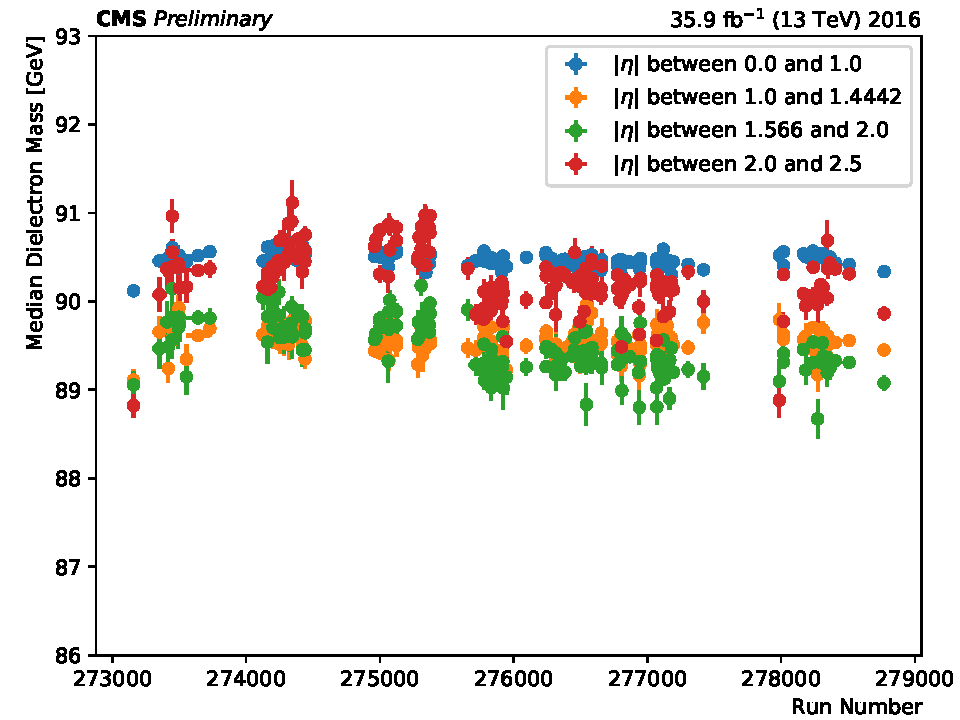
\includegraphics[width=\textwidth]{05-figures/ul16_preVFP_step1_raw.pdf}
            \end{center}%
        \end{minipage}
    }~\subfloat{%
        \begin{minipage}[t]{0.5\textwidth}%
            \begin{center}
            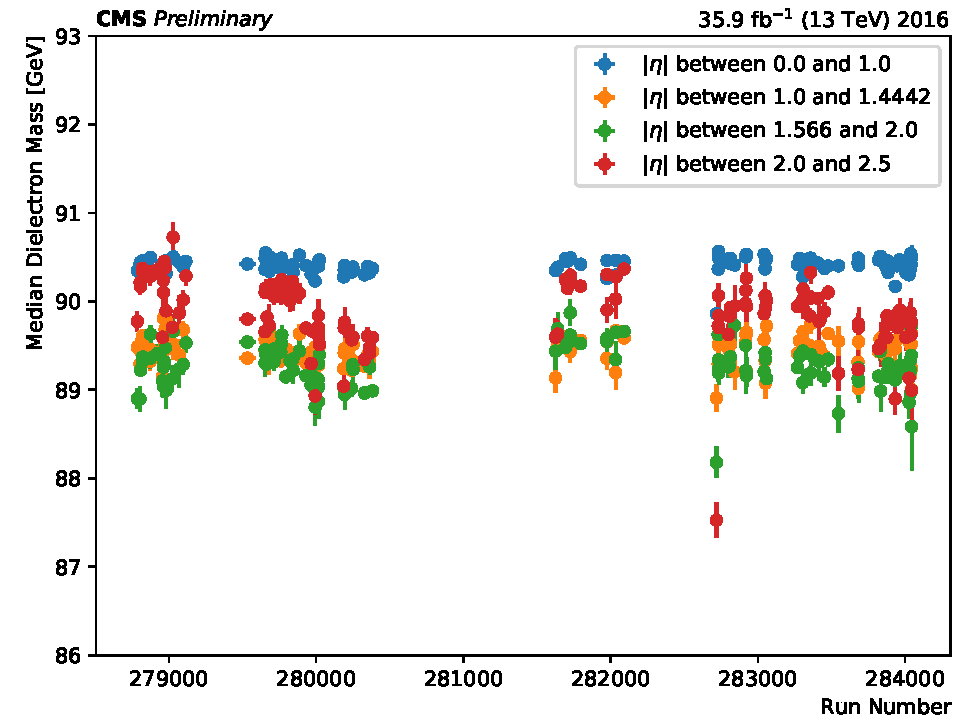
\includegraphics[width=\textwidth]{05-figures/ul16_postVFP_step1_raw.pdf}
            \end{center}
        \end{minipage}
    }~\subfloat{%
        \begin{minipage}[t]{0.5\textwidth}%
            \begin{center}
            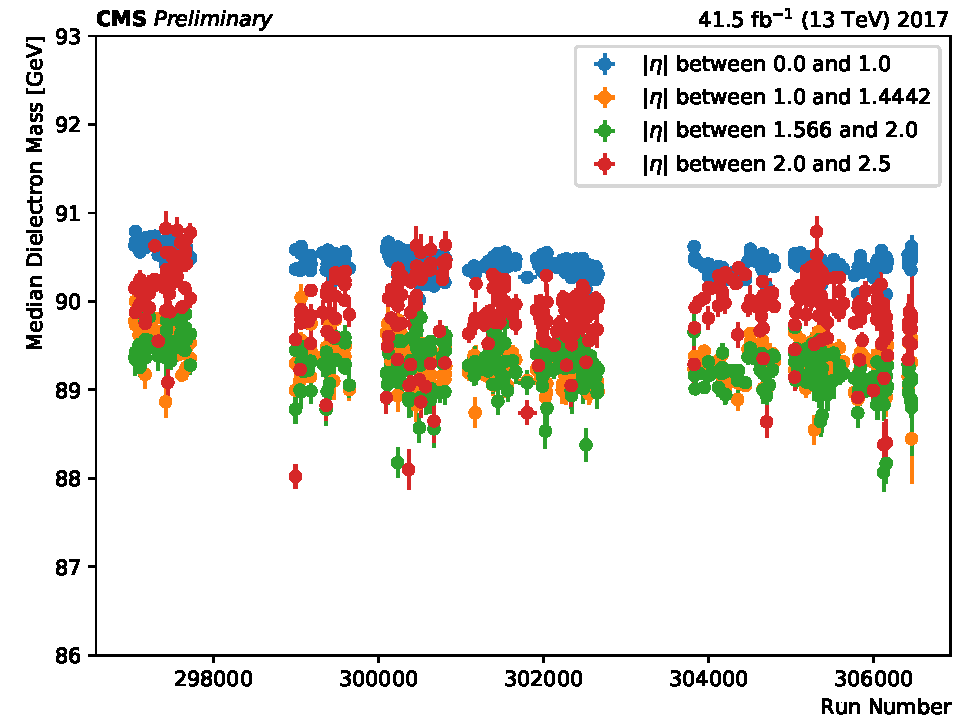
\includegraphics[width=\textwidth]{05-figures/ul17_step1_raw.pdf}
            \end{center}
        \end{minipage}
    }~\subfloat{%
        \begin{minipage}[t]{0.5\textwidth}%
            \begin{center}
            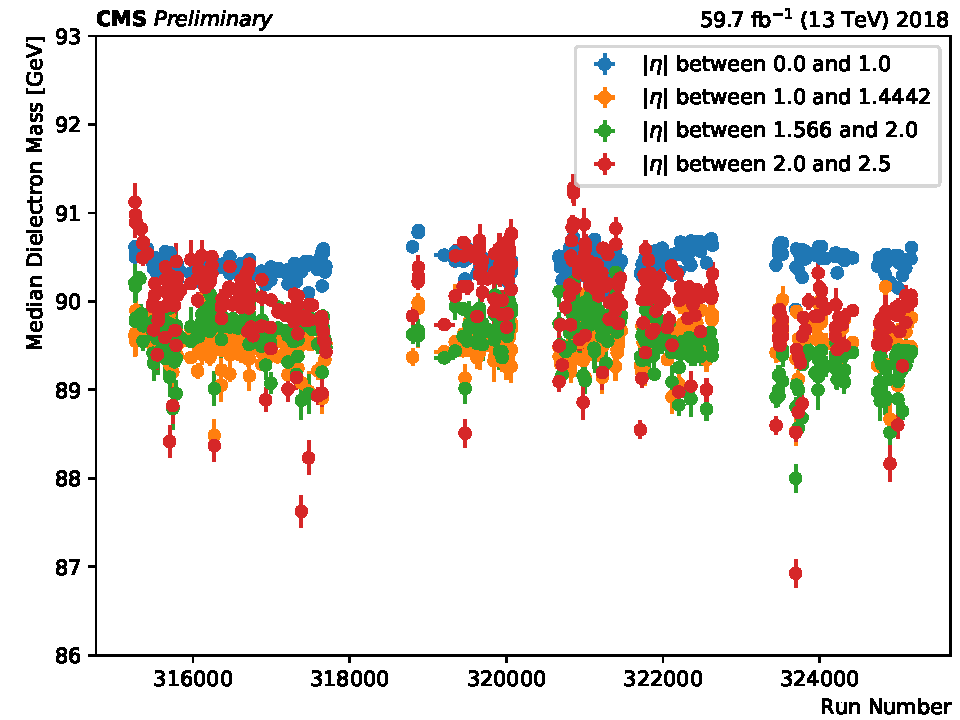
\includegraphics[width=\textwidth]{05-figures/ul18_step1_raw.pdf}
            \end{center}
        \end{minipage}
    }
    \caption[Before run dependent scales: 2016, 2017, 2018]{Z lineshape peak values in 2016 preVFP (top left), 2016 postVFP (top right), 2017 (bottom left), and 2018 (bottom right) datasets in bins of run number and $\eta$ for 2016.}
    \label{fig:before_step1_corrections}
\end{figure}


As described above, we apply the ``median method" to the data to correct the median dielectron invariant mass to the PDG value of Z mass. The corrected median dielectron invariant mass is shown for the 2016, 2017, and 2018 datasets in Figure~\ref{fig:after_step1_corrections}.


\begin{figure}[hbtp]
    \subfloat{%
        \begin{minipage}[t]{0.5\textwidth}%
            \begin{center}
                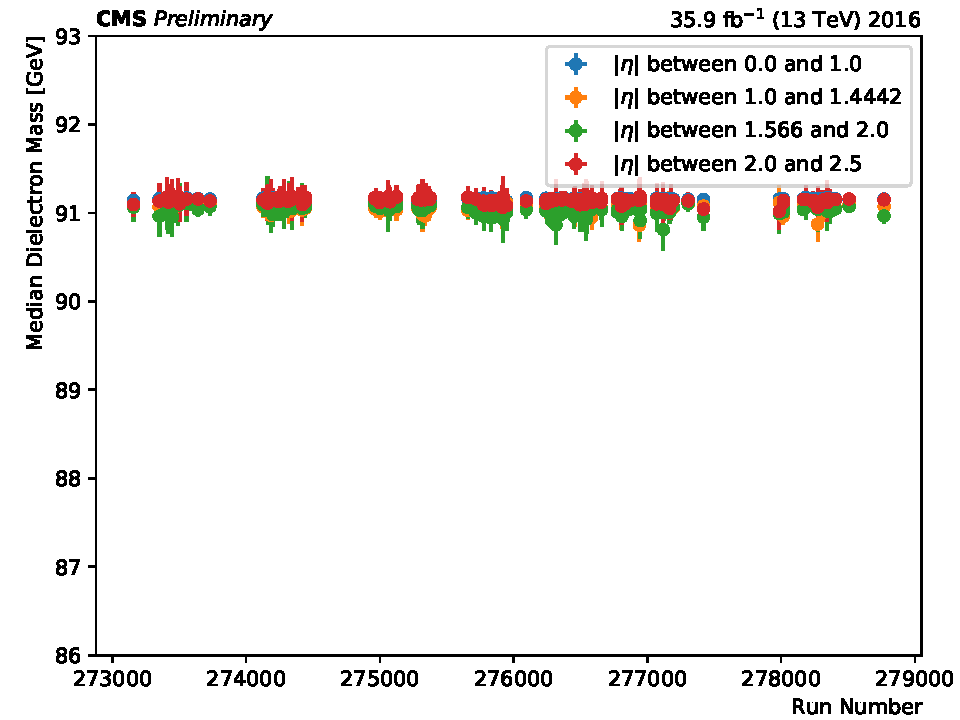
\includegraphics[width=\textwidth]{05-figures/ul16_preVFP_step1_closure.pdf}
            \end{center}%
        \end{minipage}
    }~\subfloat{%
        \begin{minipage}[t]{0.5\textwidth}%
            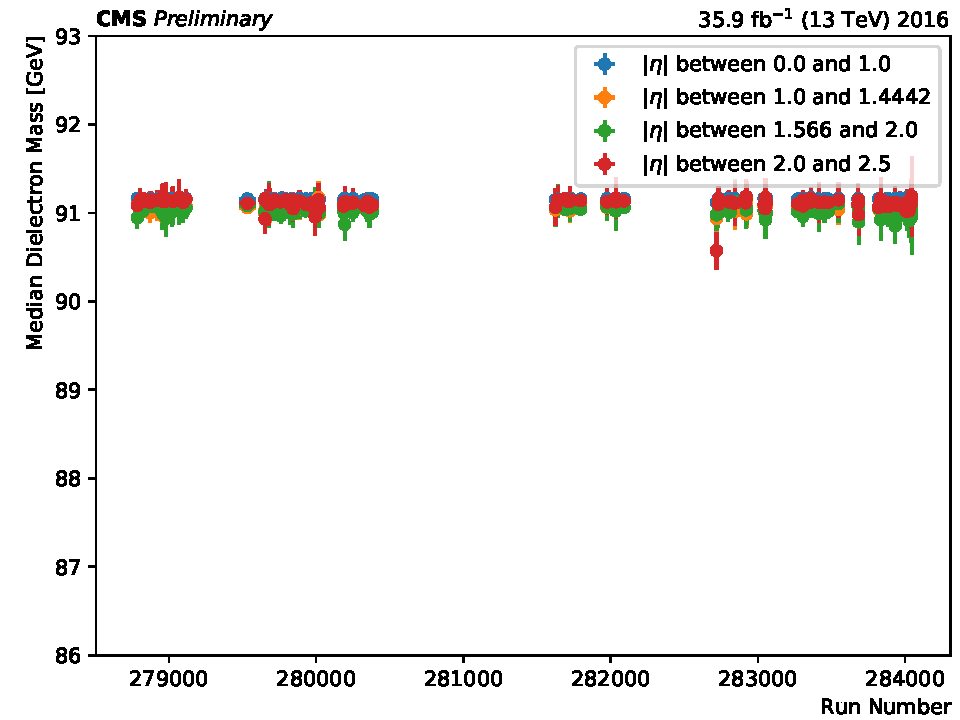
\includegraphics[width=\textwidth]{05-figures/ul16_postVFP_step1_closure.pdf}
        \end{minipage}
    }~\subfloat{%
        \begin{minipage}[t]{0.5\textwidth}%
            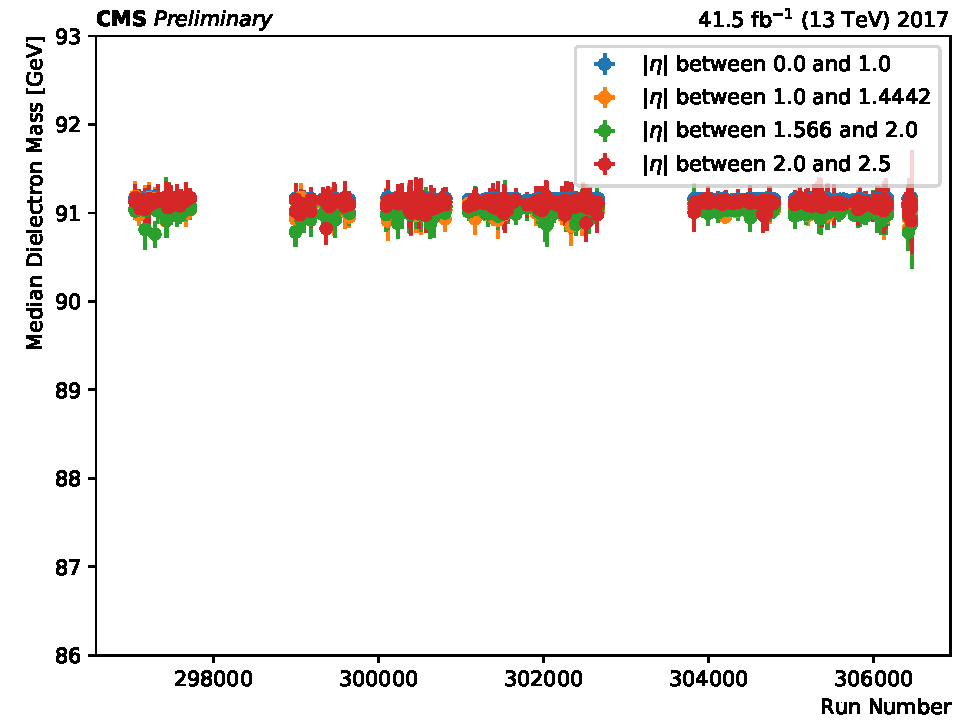
\includegraphics[width=\textwidth]{05-figures/ul17_step1_closure.pdf}
        \end{minipage}
    }~\subfloat{%
        \begin{minipage}[t]{0.5\textwidth}%
            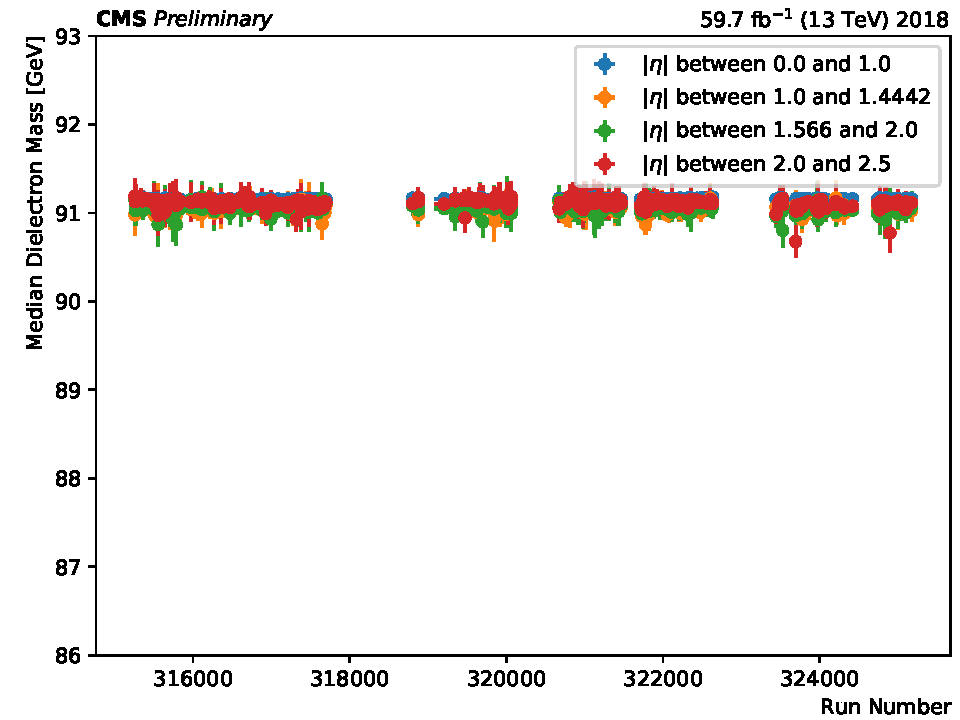
\includegraphics[width=\textwidth]{05-figures/ul18_step1_closure.pdf}
        \end{minipage}
    }
    \caption[After run dependent scales: 2016, 2017, 2018]{Z lineshape peak values in 2016 preVFP (top left), 2016 postVFP (top right), 2017 (bottom left), and 2018 (bottom right) datasets after step 1 corrections in bins of run number and $|\eta|$.}
    \label{fig:after_step1_corrections}
\end{figure}


\subsection{$E_T$ dependent residual scales and additional smearings}
\label{subsec:et_scales}

After applying the run-dependent corrections, the residual scales and additional smearings are derived simultaneously using the ``global smearing method" in 10-13 bins in R$_{9}$ and 5 in $|\eta|$. By binning finely in R$_{9}$, the corrections become independent of the effective R$_{9}$ distributions in this analysis' categories. These corrections for the 2017 dataset are shown for the EB and EE in Figure~\ref{fig:ul17_step3}. The smearings for this set of corrections are derived in coarser bins of $|\eta|$ and R$_{9}$ with four bins in $|\eta|$ and two bins in R$_{9}$.

\begin{figure}[h]
    \subfloat{%
    \begin{minipage}[t]{0.49\textwidth}%
        \centering
        \includegraphics[width=\textwidth]{05-figures/ul17_step3_eb.png}
    \end{minipage}
    }~\subfloat{%
    \begin{minipage}[t]{0.49\textwidth}%
        \centering
        \includegraphics[width=\textwidth]{05-figures/ul17_step3_ee.png}
    \end{minipage}
    }
    \centering
    \caption[Scales as a function of R$_9$]{The residual scale in \% as a function of R$_9$ as derived for the 2017 dataset in the EB (left) and EE (right).}
    \label{fig:ul17_step3}
\end{figure}


In Run 1, a set of $E_T$ dependent smearings was derived to correct for differences in resolution as a function of the energy of the electrons. These smearings were derived by decoupling the constant term smearing from the stochastic term smearing using an angle $\phi$. Using the GSM, we derive the stochastic term as a constant term with constraints on $E_T$. This approach yields stable stochastic smearings, which are more stable than the Run 1 approach. The increased stability also comes with smaller uncertainties on the stochastic smearings. A set of scales and stochastic smearings were derived for the electron energy using the GMS in four bins of $|eta|$, four bins of E$_T$, and two bins of R$_9$. These scales and smearings were derived to account for the differences in resolution as a function of energy and have yielded greatly improved agreement in data and simulation. The final smearings for 2016, 2017, and 2018 are listed in Table~\ref{tab:stochasticSmearings_Run2}.


\begin{table}{ c p{10cm}}[htbp]
    \centering    
    \small
    \setlength\tabcolsep{2pt}
    \caption[Additional Gaussian smearings ($\Delta\sigma$) in percent]{Additional Gaussian smearings ($\Delta\sigma$) in percent applied to 2016 preVFP, 2016 postVFP, 2017, and 2018 simulations.}
    \begin{tabular}{|c  c  c | c | c | c | c |}
    \hline
        $|\eta|$ & R$_{9}$ & E$_{T}$ [GeV] & 2016 preVFP & 2016 postVFP & 2017 & 2018\\ \hline \hline
        0 $\leq |\eta| <$ 1 & R$_{9}$ $< 0.96$ & 20 $\leq$ E$_T$ $<$ 39      & 1.29 & 1.44 & 1.59 & 1.54 \\ \hline
        &  & 39 $\leq$ E$_T$ $<$ 50                                          & 0.87 & 0.92 & 1.04 & 0.90 \\ \hline
        &  & 50 $\leq$ E$_T$ $<$ 65                                          & 0.00 & 0.07 & 0.03 & 0.55 \\ \hline
        &  & 65 $\leq$ E$_T$                                                 & 0.00 & 0.02 & 0.07 & 0.76 \\ \hline
        & R$_{9}$ $> 0.96$ & 20 $\leq$ E$_T$ $<$ 39                          & 1.40 & 1.38 & 1.45 & 1.18 \\ \hline
        &  & 39 $\leq$ E$_T$ $<$ 50                                          & 0.47 & 0.36 & 0.45 & 0.49 \\ \hline
        &  & 50 $\leq$ E$_T$ $<$ 65                                          & 0.13 & 0.00 & 0.01 & 0.57 \\ \hline
        &  & 65 $\leq$ E$_T$                                                 & 0.02 & 0.00 & 0.10 & 0.56 \\ \hline
        1 $\leq |\eta| <$ 1.4442 & R$_{9}$ $< 0.96$ & 20 $\leq$ E$_T$ $<$ 39 & 1.55 & 1.80 & 1.93 & 0.50 \\ \hline
        &  & 39 $\leq$ E$_T$ $<$ 50                                          & 1.58 & 1.92 & 2.20 & 2.24 \\ \hline
        &  & 50 $\leq$ E$_T$ $<$ 65                                          & 0.82 & 1.34 & 0.35 & 1.60 \\ \hline
        &  & 65 $\leq$ E$_T$                                                 & 1.01 & 1.23 & 1.50 & 1.97 \\ \hline
        & R$_{9}$ $> 0.96$ & 20 $\leq$ E$_T$ $<$ 39                          & 0.82 & 1.14 & 1.50 & 1.21 \\ \hline
        &  & 39 $\leq$ E$_T$ $<$ 50                                          & 1.30 & 1.47 & 1.30 & 1.20 \\ \hline
        &  & 50 $\leq$ E$_T$ $<$ 65                                          & 0.79 & 0.41 & 0.02 & 0.70 \\ \hline
        &  & 65 $\leq$ E$_T$                                                 & 0.56 & 0.48 & 0.80 & 1.23 \\ \hline
        1.566 $\leq |\eta| <$ 2 & R$_{9}$ $< 0.96$ & 20 $\leq$ E$_T$ $<$ 39  & 1.27 & 1.53 & 2.00 & 0.58 \\ \hline
        &  & 39 $\leq$ E$_T$ $<$ 50                                          & 1.13 & 1.33 & 1.85 & 2.25 \\ \hline
        &  & 50 $\leq$ E$_T$ $<$ 65                                          & 1.35 & 1.46 & 1.67 & 2.12 \\ \hline
        &  & 65 $\leq$ E$_T$                                                 & 2.16 & 1.64 & 2.22 & 2.38 \\ \hline
        & R$_{9}$ $> 0.96$ & 20 $\leq$ E$_T$ $<$ 39                          & 0.68 & 0.66 & 1.48 & 1.51 \\ \hline
        &  & 39 $\leq$ E$_T$ $<$ 50                                          & 0.76 & 0.91 & 1.23 & 1.38 \\ \hline
        &  & 50 $\leq$ E$_T$ $<$ 65                                          & 1.35 & 1.02 & 1.62 & 1.39 \\ \hline
        &  & 65 $\leq$ E$_T$                                                 & 1.44 & 1.10 & 1.60 & 1.45 \\ \hline
        2 $\leq |\eta| <$ 2.5 & R$_{9}$ $< 0.96$ & 20 $\leq$ E$_T$ $<$ 39    & 0.02 & 1.13 & 1.60 & 0.16 \\ \hline
        &  & 39 $\leq$ E$_T$ $<$ 50                                          & 0.81 & 0.93 & 1.50 & 1.89 \\ \hline
        &  & 50 $\leq$ E$_T$ $<$ 65                                          & 1.30 & 1.39 & 1.70 & 2.09 \\ \hline
        &  & 65 $\leq$ E$_T$                                                 & 1.41 & 1.55 & 2.11 & 1.90 \\ \hline
        & R$_{9}$ $> 0.96$ & 20 $\leq$ E$_T$ $<$ 39                          & 0.00 & 0.00 & 0.80 & 0.03 \\ \hline
        &  & 39 $\leq$ E$_T$ $<$ 50                                          & 0.00 & 0.00 & 0.97 & 0.70 \\ \hline
        &  & 50 $\leq$ E$_T$ $<$ 65                                          & 0.00 & 0.00 & 1.34 & 0.91 \\ \hline
        &  & 65 $\leq$ E$_T$                                                 & 0.00 & 0.00 & 2.03 & 1.59 \\ \hline
    \end{tabular}
    \label{tab:stochasticSmearings_Run2}
\end{table}


The systematic uncertainty associated with the scales and smearings that account for the variations in R$_9$, electron identification, pre-selection E$_T$ threshold, and non-closure are all added in quadrature. The details of this study are given in Chapter~\ref{chap:stats}. The agreement between data and MC after all corrections is shown for electrons with R$_9 > 0.96$ in the barrel-barrel and barrel-endcap categories for the 2016 preVFP dataset in Figure~\ref{fig:invmass_2016_prevfp}, the 2016 postVFP dataset in Figure~\ref{fig:invmass_2016_postvfp}, the 2017 dataset in Figure~\ref{fig:invmass_2017}, and the 2018 dataset in Figure~\ref{fig:invmass_2018}.

\begin{figure}[h]
    \subfloat{%
    \begin{minipage}[t]{0.49\textwidth}%
        \centering
        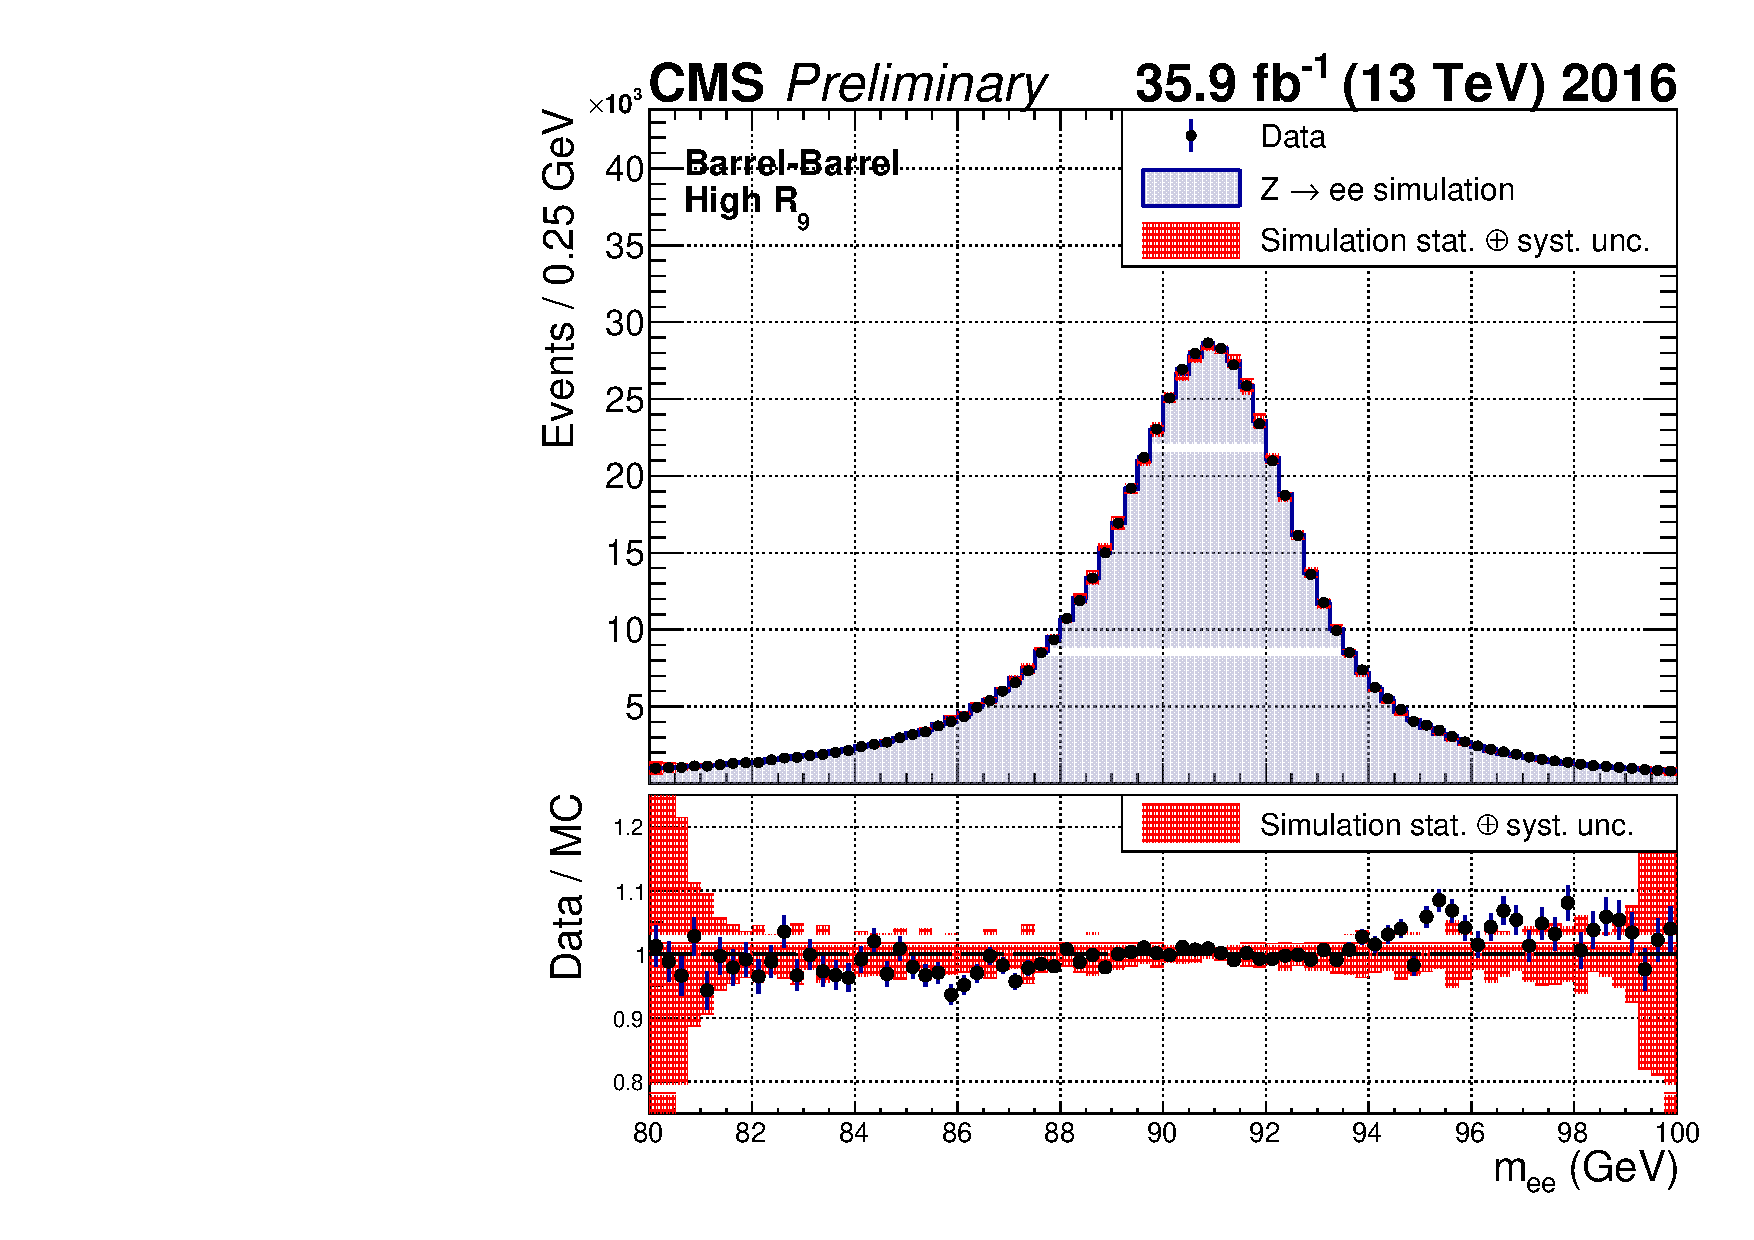
\includegraphics[width=\textwidth]{05-figures/invmass_ul16_prevfp_eb_highR9_wRatioPad.pdf}
    \end{minipage}
    }~\subfloat{%
    \begin{minipage}[t]{0.49\textwidth}%
        \centering
        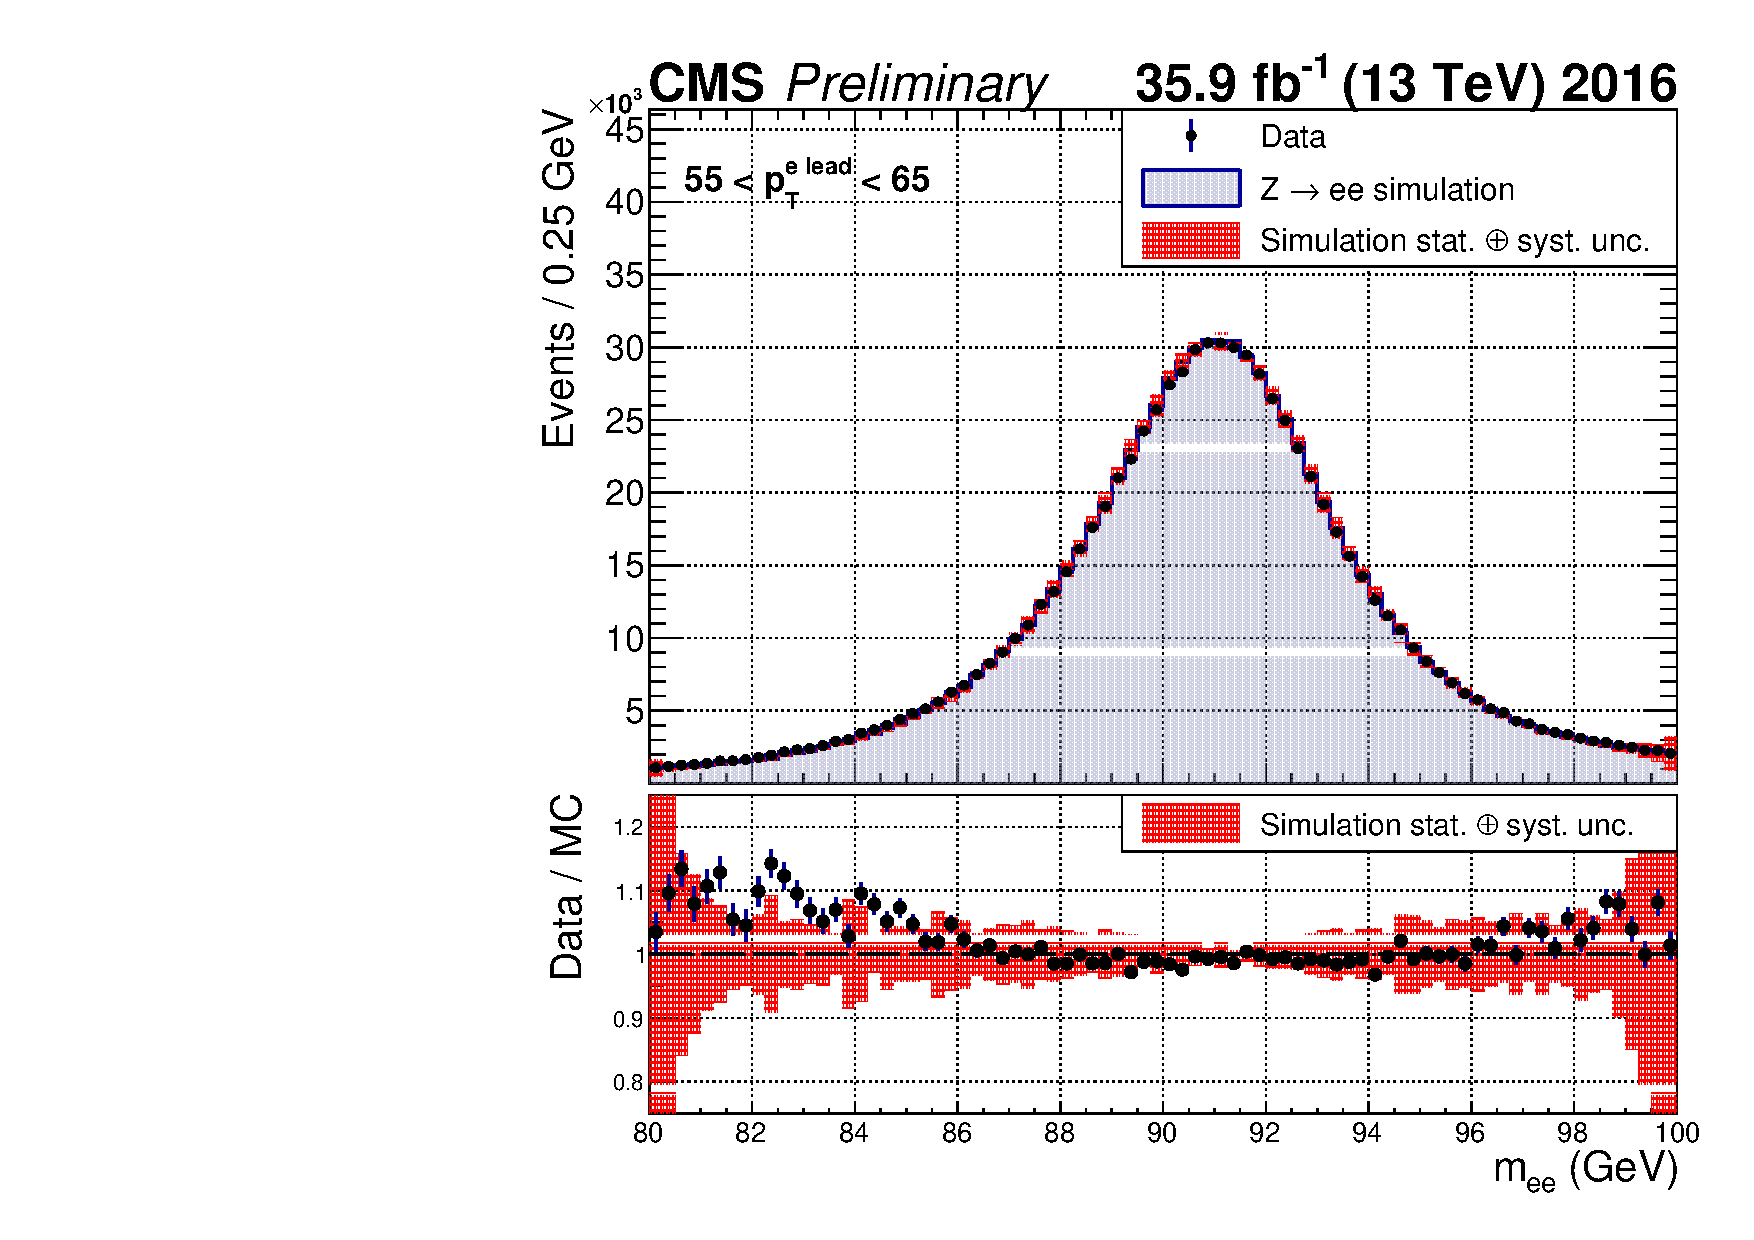
\includegraphics[width=\textwidth]{05-figures/invmass_ul16_prevfp_pt_55_65_wRatioPad.pdf}
    \end{minipage}
    }
    \centering
    \caption[Agreement in data/MC: 2016 preVFP]{Agreement in data and MC for the 2016 preVFP dataset. Shown on the left is the Barrel-Barrel, R$_9 > 0.96$ category, and on the right is the 55 GeV$ < P_{T}^{lead\ e} < $ 65 GeV category.}
    \label{fig:invmass_2016_prevfp}
\end{figure}

\begin{figure}[h]
\subfloat{%
    \begin{minipage}[t]{0.49\textwidth}%
        \centering
        \includegraphics[width=\textwidth]{05-figures/invmass_ul16_postvfp_eb_highR9_wRatioPad.pdf}
    \end{minipage}
    }~\subfloat{%
    \begin{minipage}[t]{0.49\textwidth}%
        \centering
        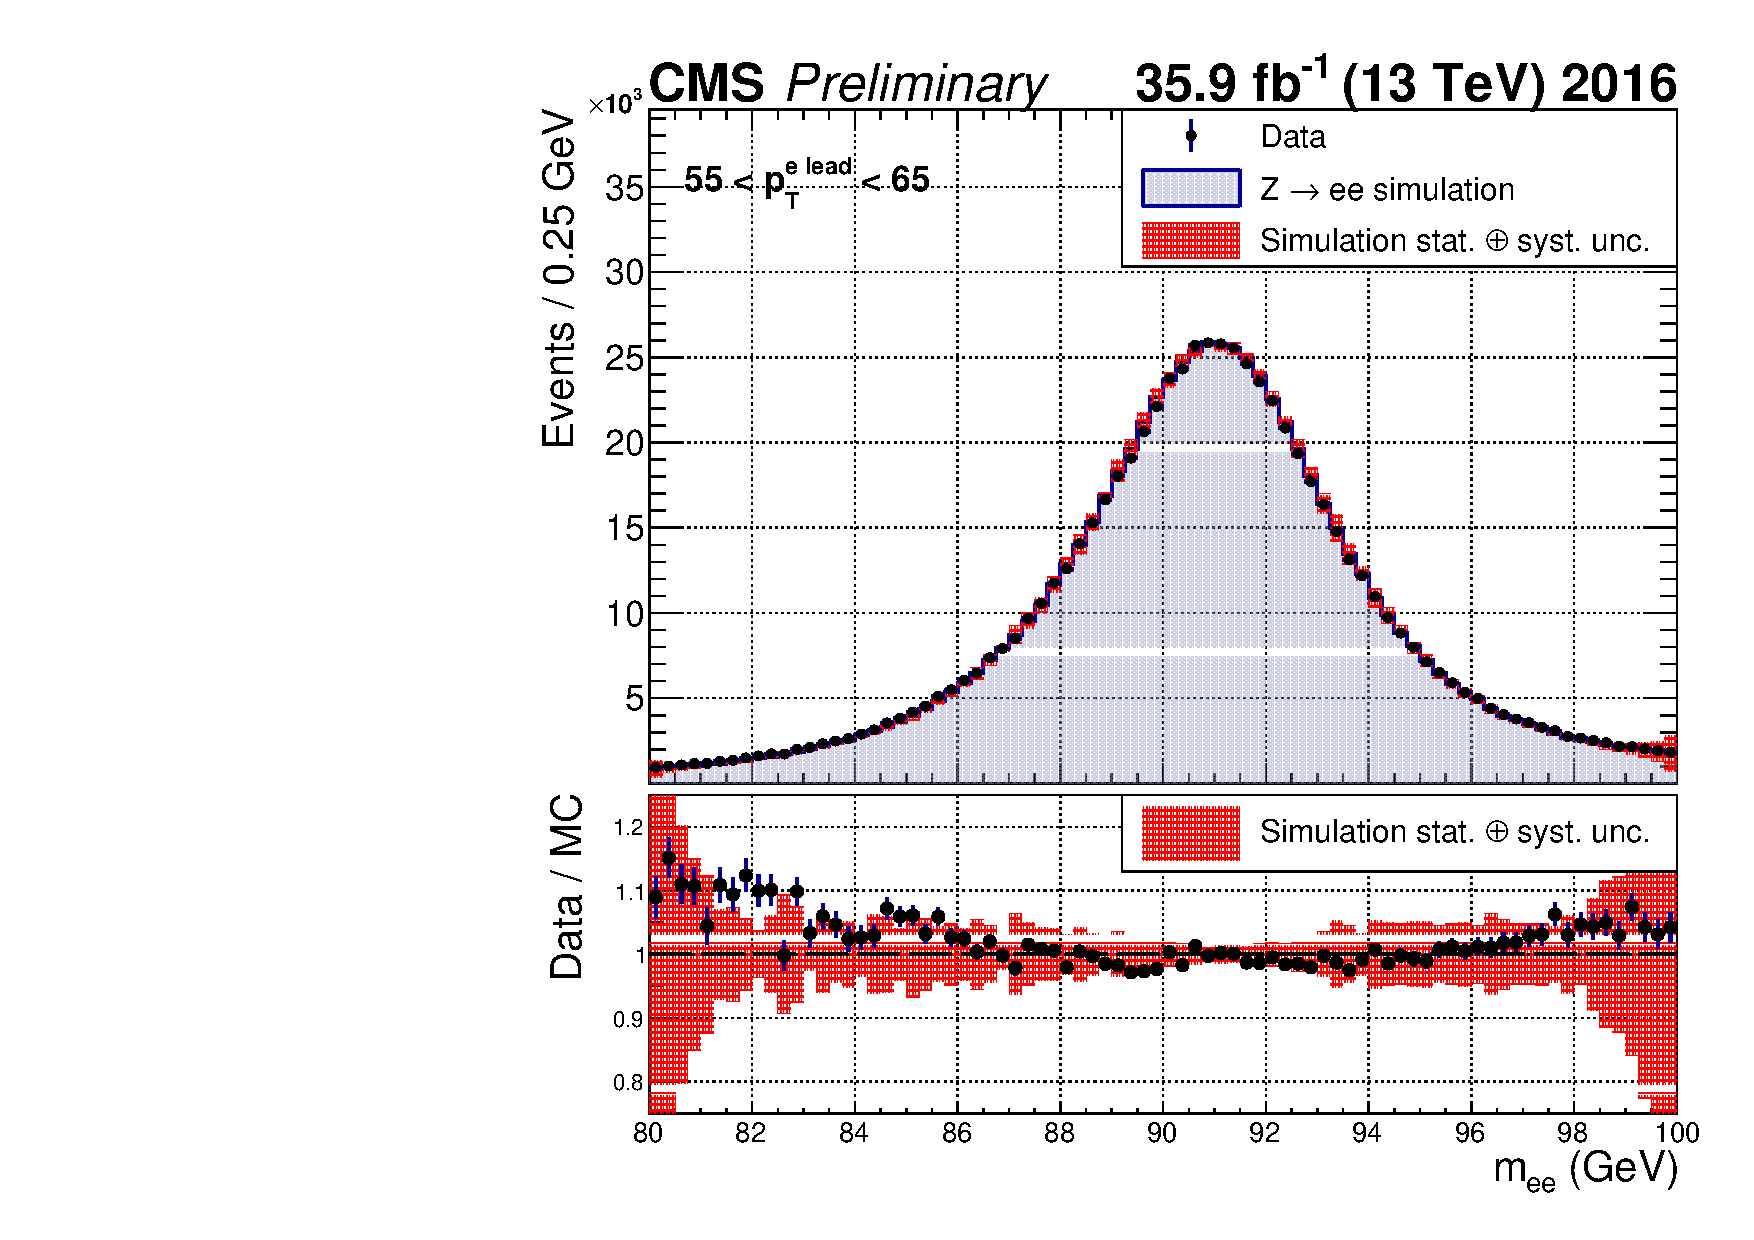
\includegraphics[width=\textwidth]{05-figures/invmass_ul16_postvfp_pt_55_65_wRatioPad.pdf}
    \end{minipage}
    }
    \centering
    \caption[Agreement in data/MC: 2016 postVFP]{Agreement in data and MC for the 2016 postVFP dataset. Shown on the left is the Barrel-Barrel, R$_9 > 0.96$ category, and on the right is the 55 GeV $< P_{T}^{lead\ e} <$ 65 GeV category.}
    \label{fig:invmass_2016_postvfp}
\end{figure}

\begin{figure}[h]
\subfloat{%
    \begin{minipage}[t]{0.49\textwidth}%
        \centering
        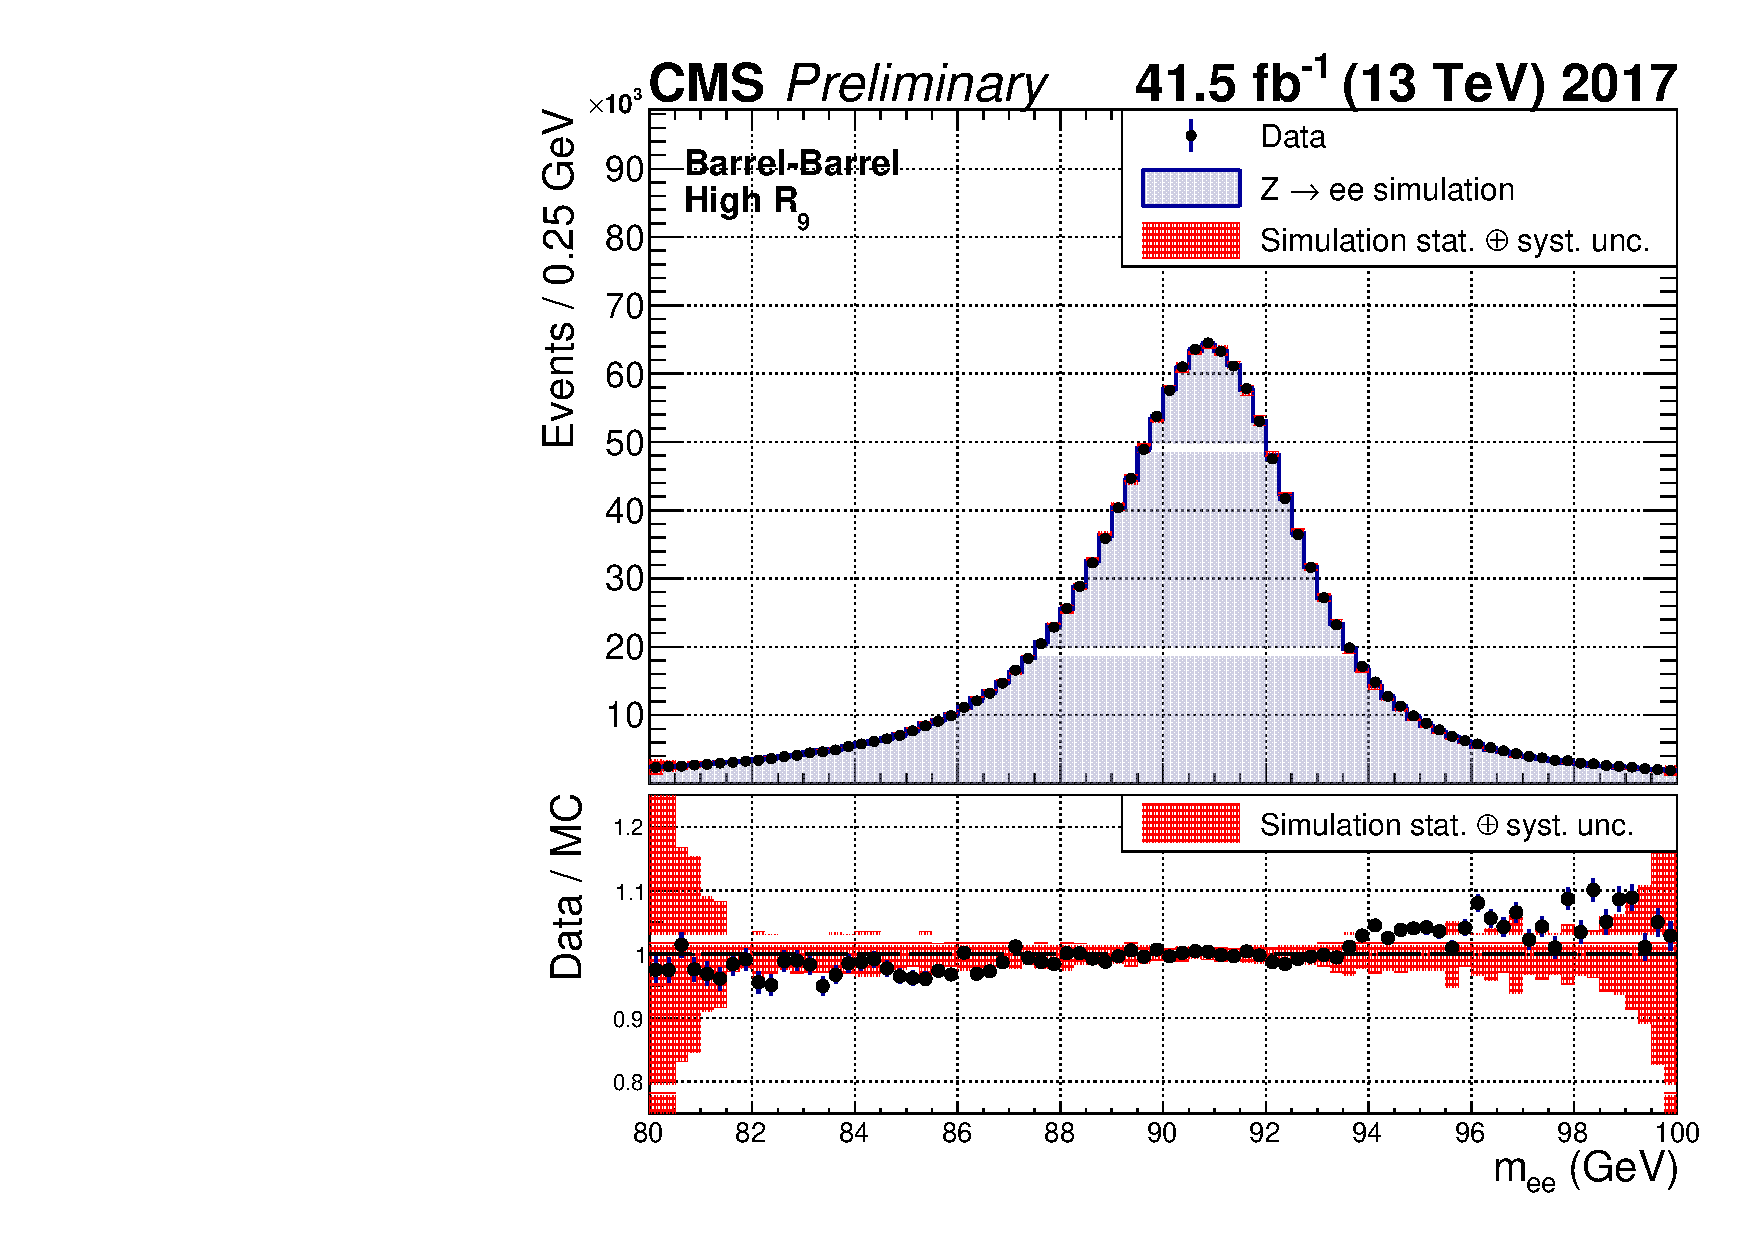
\includegraphics[width=\textwidth]{05-figures/invmass_ul17_EB_highR9_wRatioPad.pdf}
    \end{minipage}
    }~\subfloat{%
    \begin{minipage}[t]{0.49\textwidth}%
        \centering
        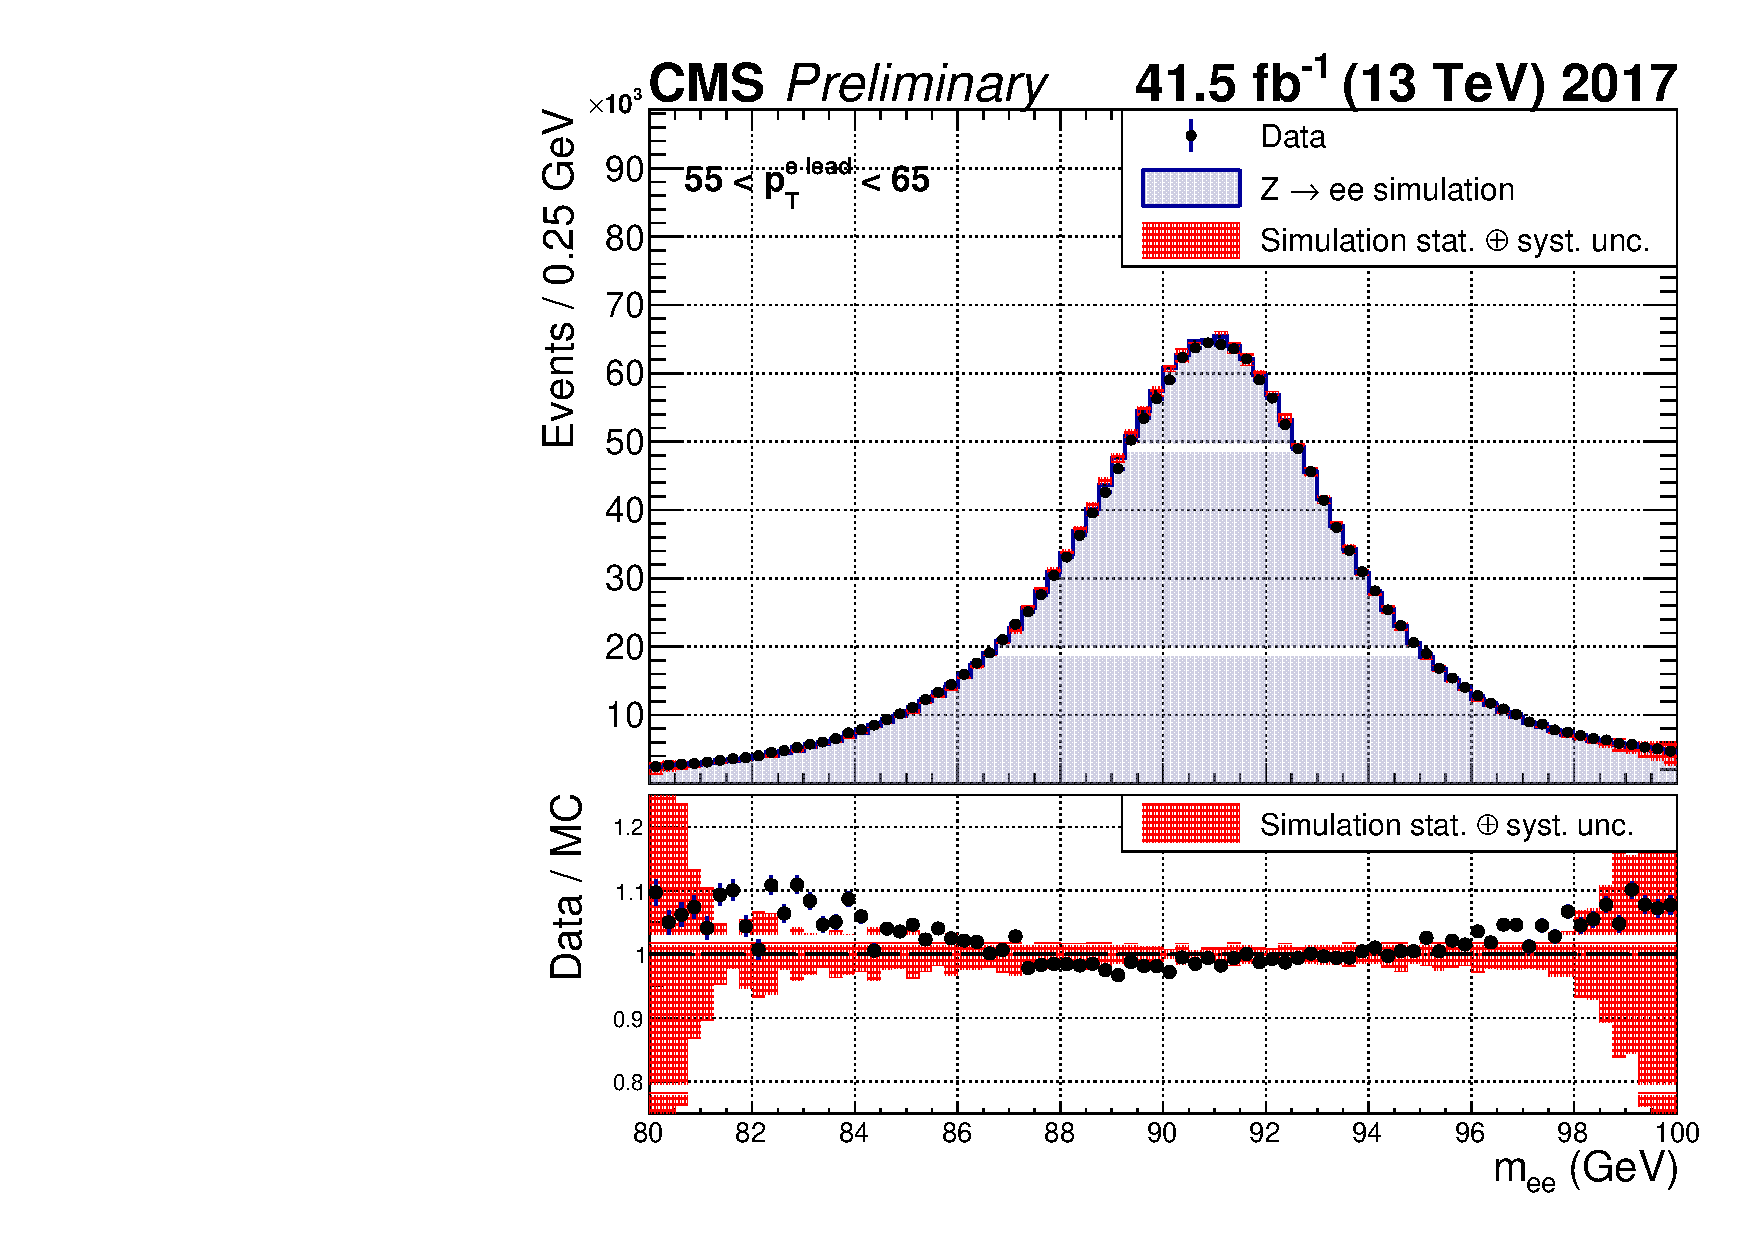
\includegraphics[width=\textwidth]{05-figures/invmass_ul17_pt_55_65_wRatioPad.pdf}
    \end{minipage}
    }
    \centering
    \caption[Agreement in data/MC: 2017]{Agreement in data and MC for the 2017 dataset. Shown on the left is the Barrel-Barrel, R$_9 > 0.96$ category, and on the right is the 55 GeV $< P_{T}^{lead\ e} <$ 65 GeV category.}
    \label{fig:invmass_2017}
\end{figure}

\begin{figure}[h]
\subfloat{%
    \begin{minipage}[t]{0.49\textwidth}%
        \centering
        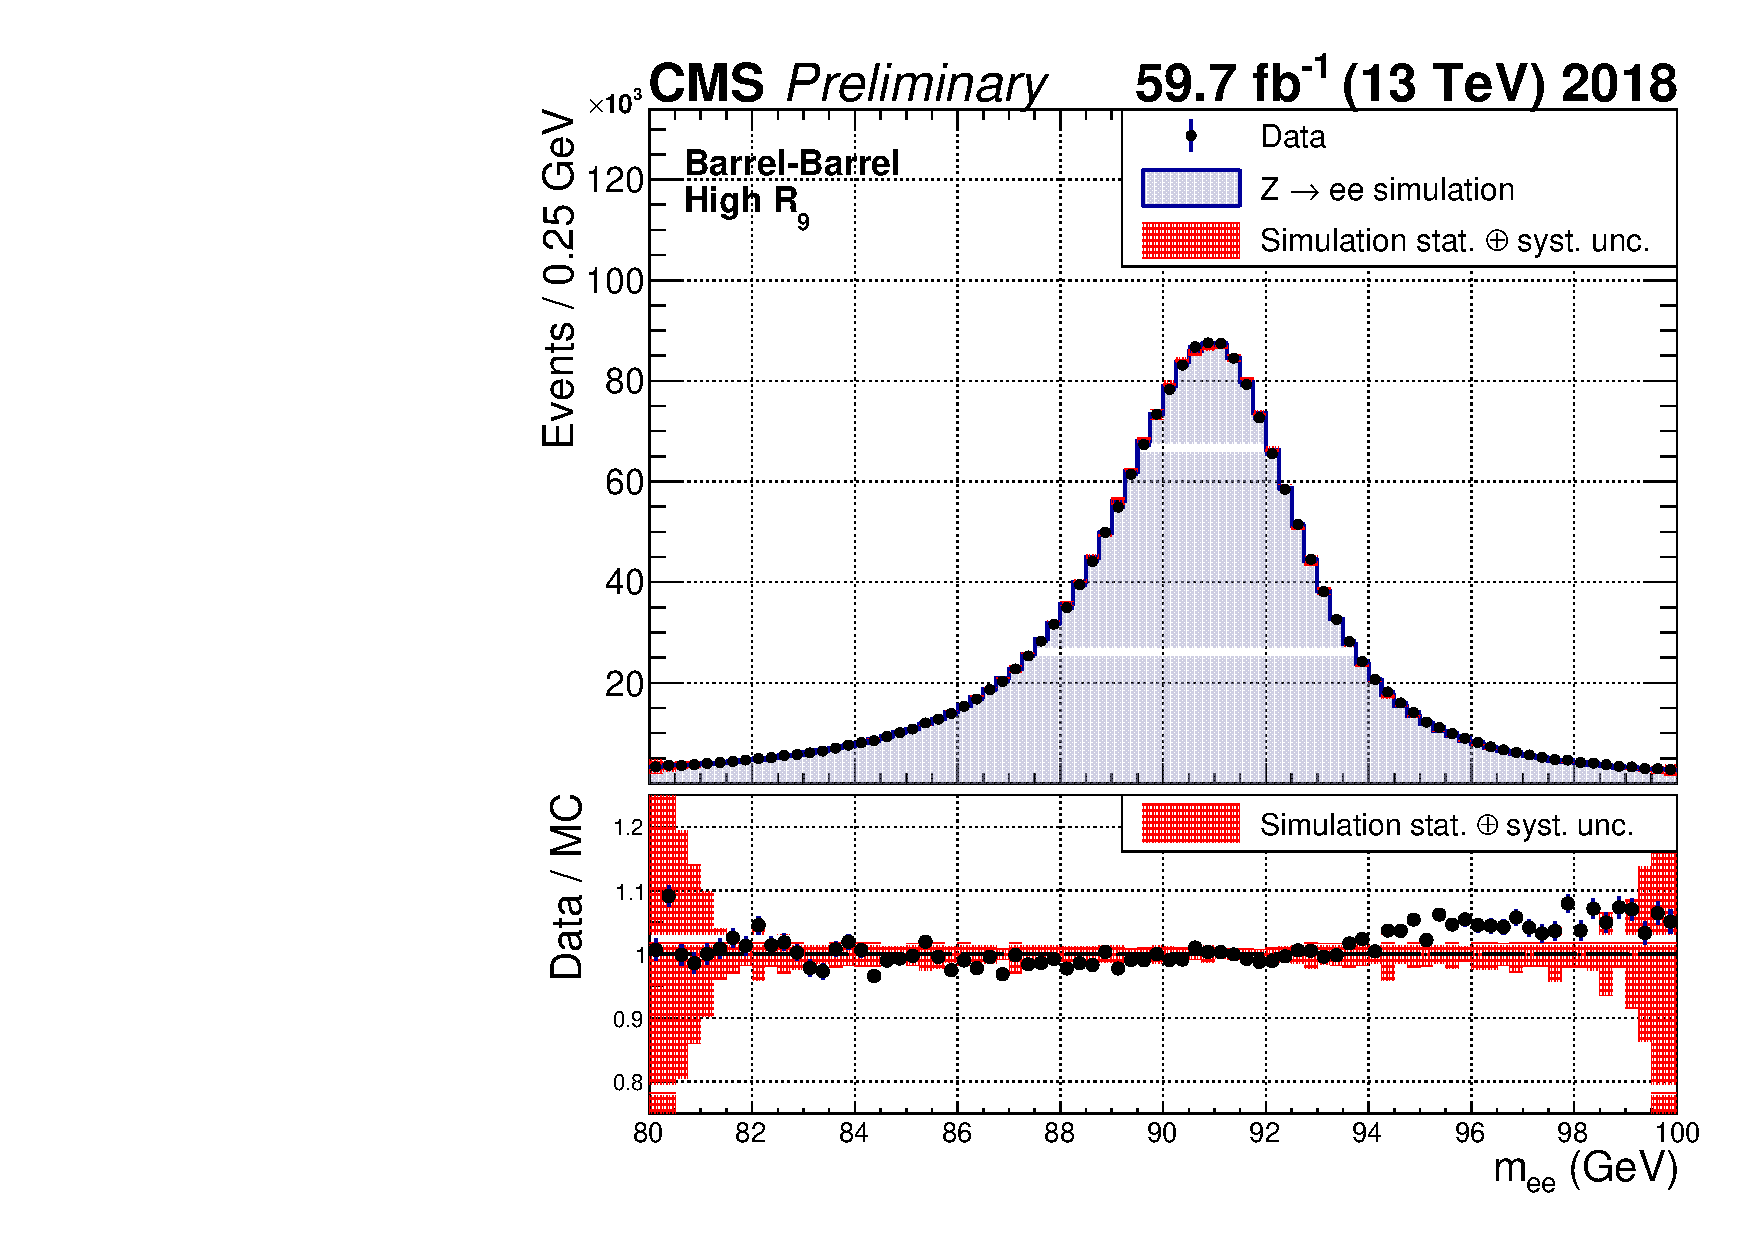
\includegraphics[width=\textwidth]{05-figures/invmass_ul18_EB_highR9_wRatioPad.pdf}
    \end{minipage}
    }~\subfloat{%
    \begin{minipage}[t]{0.49\textwidth}%
        \centering
        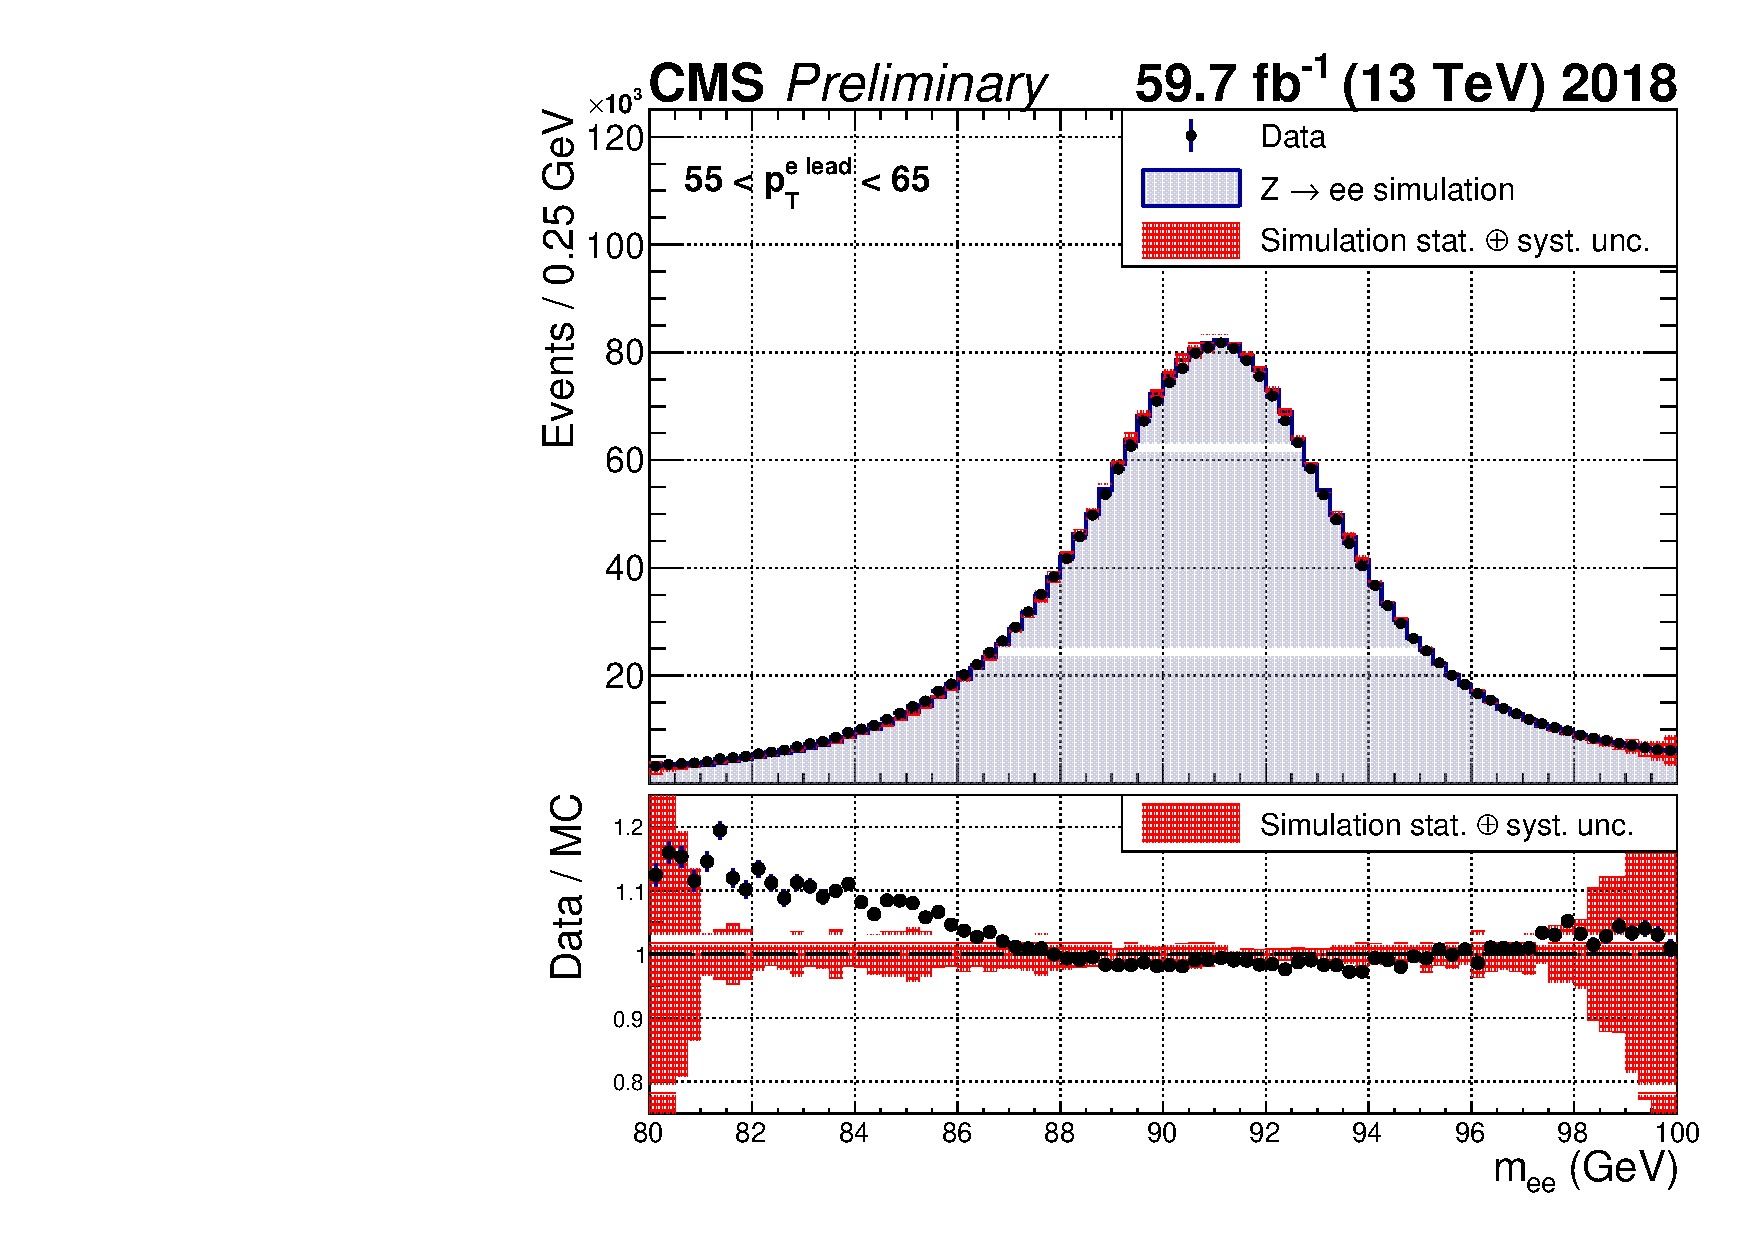
\includegraphics[width=\textwidth]{05-figures/invmass_ul18_pt_55_65_wRatioPad.pdf}
    \end{minipage}
    }
    \centering
    \caption[Agreement in data/MC: 2018]{Agreement in data and MC for the UL 2018 dataset. Shown on the left is the Barrel-Barrel, $R_9 > 0.96$ category, and on the right is the 55 GeV $< P_{T}^{lead\ e} <$ 65 GeV category.}
    \label{fig:invmass_2018}
\end{figure}